\documentclass[cjk,slidestop,compress,mathserif,blue]{beamer}
%dvipdfm选项是关键,否则编译统统通不过
%beamer的颜色选项定义的是导航条和标题的颜色(即关键词structure的颜色)

%%%%%%%%%%%%%%%%仅限于XeTeX可使用的宏包%%%%%%%%%%%%%%%%%%%%%%%%%%%%
\usepackage{fontspec,xunicode,xltxtra,beamerthemesplit}
\usepackage{beamerthemesplit}
\setsansfont[Mapping=tex-text]{Adobe 黑体 Std}
%如果装了Adobe Acrobat,可在font.conf中配置Adobe字体的路径以使用其中文字体
%也可直接使用系统中的中文字体如SimSun,SimHei,微软雅黑 等
%原来beamer用的字体是sans family;注意Mapping的大小写,不能写错

%%%%%%%%   确定标题和导航条结构的框架     %%%%%%%%%%%%
\usepackage{beamerthemeshadow}                      %
%\usepackage{beamerthemeclassic}%导航条色与背景色一致%
%%%%%%%%%%%%%%%%%%%%%%%%%%%%%%%%%%%%%%%%%%%%%%%%%%%%%%
\setbeamerfont{roman title}{size={}}
\usepackage{xeCJK} % seperate the english and chinese		 %
\usepackage{amsmath,amsthm,amsfonts,amssymb,bm}
\usepackage{mathrsfs}
\usepackage{xcolor}                                        %使用默认允许使用颜色
\usepackage{hyperref}
\usepackage{graphicx}
\usepackage{epsfig,graphics,subfigure,psfrag}

%\usepackage[numbers,sort&compress]{natbib} %紧密排列             %
\usepackage[sectionbib]{chapterbib}        %每章节单独参考文献   %
\usepackage{hypernat}                                                                         %
%\usepackage[dvipdfm,bookmarksopen=true,pdfstartview=FitH,CJKbookmarks]{hyperref}		%
\hypersetup{bookmarksnumbered,colorlinks,linkcolor=brown,citecolor=blue,urlcolor=red}         %
%参考文献含有超链接引用时需要下列宏包,注意与natbib有冲突        %
%\usepackage[dvipdfm]{hyperref}                                  %
%\usepackage{hypernat}                                           %
\newcommand{\upcite}[1]{\hspace{0ex}\textsuperscript{\cite{#1}}} %

%\useoutertheme{smoothbars}
\useinnertheme[shadow=true]{rounded}
\usetheme{Berkeley}                                          %主题式样
%\usetheme{Luebeck}

\usecolortheme{lily}                                        %颜色主题式样

\usefonttheme{professionalfonts}                           %字体主题样式宏包

%\beamertemplatetransparentcoveredhigh                      %使所有被隐藏的文本高度透明
\beamertemplatetransparentcovereddynamicmedium             %使所有被隐藏的文本完全透明,动态,动态的范围很小
\mode<presentation>
%\beamersetaveragebackground{gray}                          %设置背景颜色(单一色) 
\beamertemplateshadingbackground{green!10}{red!5}         %设置背景颜色(渐变色)

%\colorlet{mycolor}{green!60!orange}                        %定义mycolor的颜色,可放在问中的任何位置

\begin{document}
%beamer下不能用\songyi、\zihao等命令!
\graphicspath{{Figures/}}


%-------------------------------PPT Title-------------------------------------
\title{原子尺度的材料模拟软件——VASP}
%-----------------------------------------------------------------------------

%----------------------------Author & Date------------------------------------
%\author{\vskip 25pt 中物院高性能数值模拟软件中心\\\vskip 25pt 姜\quad骏}%\\\vskip 6pt\hskip 57pt黎乐民\:教授}
\author{北京市计算中心}%\quad 姜 \quad 骏\\\vskip 6pt\hskip 57pt黎乐民\:教授}
\date{\textrm{2016. 03. 29-30}}
\frame{\titlepage}
%-----------------------------------------------------------------------------

%------------------------------------------------------------------------------列出全文 outline ---------------------------------------------------------------------------------
\section*{}
\frame[allowframebreaks]
{
  \frametitle{Outline}
%  \frametitle{\textcolor{mycolor}{\secname}}
  \tableofcontents%[current,currentsection,currentsubsection]
}
%在每个section之前列出全部Outline
%类似的在每个subsection之前列出全部Outline是\AtBeginSubsection[]
\AtBeginSection[]
{
  \frame<handout:0>
  {
    \frametitle{Outline}
%全部Outline中,本部分加亮
    \tableofcontents[current,currentsection]
  }
}

%------------------------------------------------------------------------------PPT main Body------------------------------------------------------------------------------------
\small
\section{量子力学基础}
\frame
{
	\frametitle{量子力学的基本假设}
	\begin{enumerate}
		\item 微观体系的运动状态由相应的归一化波函数描述
		\item 微观体系的运动状态波函数随时间变化的规律遵从薛定谔方程
		\item 力学量由相应的线性厄米算符表示
		\item 力学量算符之间有确定的对易关系,称为量子条件;坐标算符的三个直角坐标系分量与动量算符的三个直角坐标系分量之间的对应关系称为基本量子条件;力学量算符由其相应的量子条件确定
		\item 全同的多粒子体系的波函数对于任意一对粒子交换而言具有对称性:玻色子系的波函数是对称的,费米子系的波函数是反对称的。
	\end{enumerate}
}


\section{密度泛函理论(DFT)基础}       %Bookmark
\frame                               %
{
\frametitle{密度泛函理论(\textrm{DFT})} %Slide Page Title
%   \secname
与传统的量子力学方法不同,密度泛函理论的基本变量是体系的基态电子密度。%通过体系的电子密度而非波函数确定体系的基态能量。
\begin{itemize}%[+-| alert@+>]
	\item 密度泛函理论的基石:\textrm{Hohenberg-Kohn}定理\upcite{PR136-B864_1964}
\vskip 10pt
\begin{itemize}%[+-| alert@+>]
   \setlength{\itemsep}{15pt}
 \item $E[\rho]=F_{\mathrm{HK}}[\rho]+\displaystyle\int\rho(\vec{r})v(\vec{r})\textrm{d}^{3}\vec{r}$ \\
\vskip 5pt 其中$F_{\mathrm{HK}}[\rho]=\underset{\Psi\to\rho}{\mathrm{Min}}\langle\Psi[\rho]|\hat{T}+\hat{W}|\Psi[\rho]\rangle$
是普适的泛函表达式。%,指明多电子体系的基态性质与基态密度间存在一一对应关系
     \textrm{\small{第一定理表明多电子体系的性质完全由体系的基态密度决定}}
   \item 如果$\tilde\Psi\neq\Psi$,
     $E[\tilde\rho]\geqslant E[\rho_0]$\\
     \textrm{\small{第二定理指出基态总能量泛函在体系基态电子密度处取极小值}}
   \end{itemize}
%\textrm{\small{第二定理指出基态总能量泛函在体系基态电子密度处取极小值}}
\vskip 15pt
 \item 密度泛函理论的优越性:用密度($\rho$)代替波函数($\Psi$)描述体系
\vskip 10pt
 \item 密度泛函理论的困难:能量密度泛函的精确形式未知
   \end{itemize}
}
\frame                               %
{
\frametitle{密度泛函理论(\textrm{DFT})}
\textrm{Kohn-Sham}方程\upcite{PR140-A1133_1965}:无相互作用体系+交换-相关能
$$(T_S+V_{e\!f\!f})|\varphi_i\rangle=\varepsilon_i|\varphi_i\rangle,\quad i=1,\cdots,N,\dots$$
其中$V_{e\!f\!f}(\vec r)=v(\vec r)+\displaystyle\int w(\vec r,\vec r\,')\rho(\vec r\,')d^3\vec r+\dfrac{\delta E_{XC}}{\delta\rho(\vec r)}$
\vskip 10pt
\textrm{Kohn-Sham}方程是形式上的单粒子方程
\vskip 20pt
\textrm{Kohn-Sham}方程的实质:将动能泛函的主要部分分离出来,剩余部分放在交换相关能中
}
%  \beamertemplateshadingbackground{blue!10}{yellow!10}
\frame                               %
{
\frametitle{交换-相关能密度泛函}
% \begin{itemize}%[+-| alert@+>]
%\item 交换-相关能密度泛函
\vskip 10pt
 \begin{itemize}%[+-| alert@+>]
   \setlength{\itemsep}{10pt}
 \item \textrm{LDA}:泛函只与密度分布的局域值有关
 \item \textrm{GGA}\,(包括\textrm{PW91}、\textrm{LYP}等):泛函依赖的变量:局域密度\&局域密度梯度
 \item $meta$-\textrm{GGA}\,(包括\textrm{BR89}、\textrm{B00}等):泛函依赖的变量还包括动能密度
 \item 杂化(\textrm{hybrid})泛函\,(\textrm{B3LYP}等):泛函与占据轨道有关
 \item 其他的交换-相关能泛函
 \item 完全非局域泛函:\;\;理想泛函,不现实
   \end{itemize}
   \textrm{\huge It is \textcolor{red}{Jacob's ladder}}
}

\frame                               %
{
	\frametitle{近似能量泛函$E_{\mathrm{XC}}[\rho]$的主要问题}
\vskip 20pt
\begin{enumerate}%[+-| alert@+>]
   \setlength{\itemsep}{30pt}
 \item  密度是整体变量:电子自相互作用抵消不净%\quad\textrm{(LDA+U)}方法的校正%(\textrm{LDA+U})
 \item  电子相关:简并和近简并基态能量的表示不合理
 \item  渐近行为:处理弱相互作用体系的误差大
 \end{enumerate}
}

%\section{Induction on DFT and solid-state physics}       %Bookmark
\section{固体能带理论简介}       %Bookmark
\frame
{
%\frametitle{The Bloch theorem}
\frametitle{固体能带理论}
\begin{itemize}%[+-| alert@+>]
   \setlength{\itemsep}{10pt}
   \item 固体能带理论\upcite{Huang_Han}是固体电子理论的基础,形式上是单电子理论:
    $$\hat H |\psi_i^{\vec k}(\vec r)\rangle=\bigg[-\dfrac{\hbar^2}{2m}\nabla^2+V(\vec r)\bigg]|\psi_i^{\vec k}(\vec r)\rangle=\epsilon_i(\vec k)|\psi_i^{\vec k}(\vec r)\rangle$$
  \item \textrm{\large{Bloch 定理:}}
%   \item \textrm{periodic potential:} $$V(\vec r)=V(\vec r+\vec R_n)$$
%     \textrm{Here,} $\vec R_n=n\vec R$
%   \item \textrm{Bloch theorem:}$$\psi_{\vec k}(\vec r)=\textrm{e}^{\textrm i\vec k\cdot\vec r}u_{\vec k}(\vec r)$$
%     \textrm{Here, $u_{\vec k}(\vec r)$ is a periodic function with the same periodicity as $V(\vec r)$, i.e., $u_{\vec k}(\vec r)=u_{\vec k}(\vec r+\vec R_n)$, then Bloch theorem could reads as:}
%     $$\psi_{\vec k}(\vec r+\vec R_n)=\textrm{e}^{\textrm i\vec k\cdot\vec R_n}\psi_{\vec k}(\vec r)$$
具有平移周期性的理想晶体,势能$V(\vec r)$满足$$V(\vec r)=V(\vec r+\vec R_n)$$
体系的波函数满足\textrm{Bloch}波函数形式:$$\psi_{\vec k}(\vec r)=\textrm{e}^{i\vec k\cdot\vec r}u_{\vec k}(\vec r)$$
是平面波和周期函数的乘积。$u(\vec r)$与势能有相同的周期。即$u_{\vec k}(\vec r)=u_{\vec k}(\vec r+\vec R_n)$
  \item 能带理论相当于分子轨道理论
%   \setlength{\itemsep}{30pt}
\item \textrm{Bloch}函数反映了波函数在周期性势场下的变化规律。
\end{itemize}
}

\frame
{
\frametitle{固体能带理论}
简并态微扰理论引起的能带裂分
\begin{figure}[h!]
\centering
%\hspace*{-10pt}
%\vspace*{-1.1in}
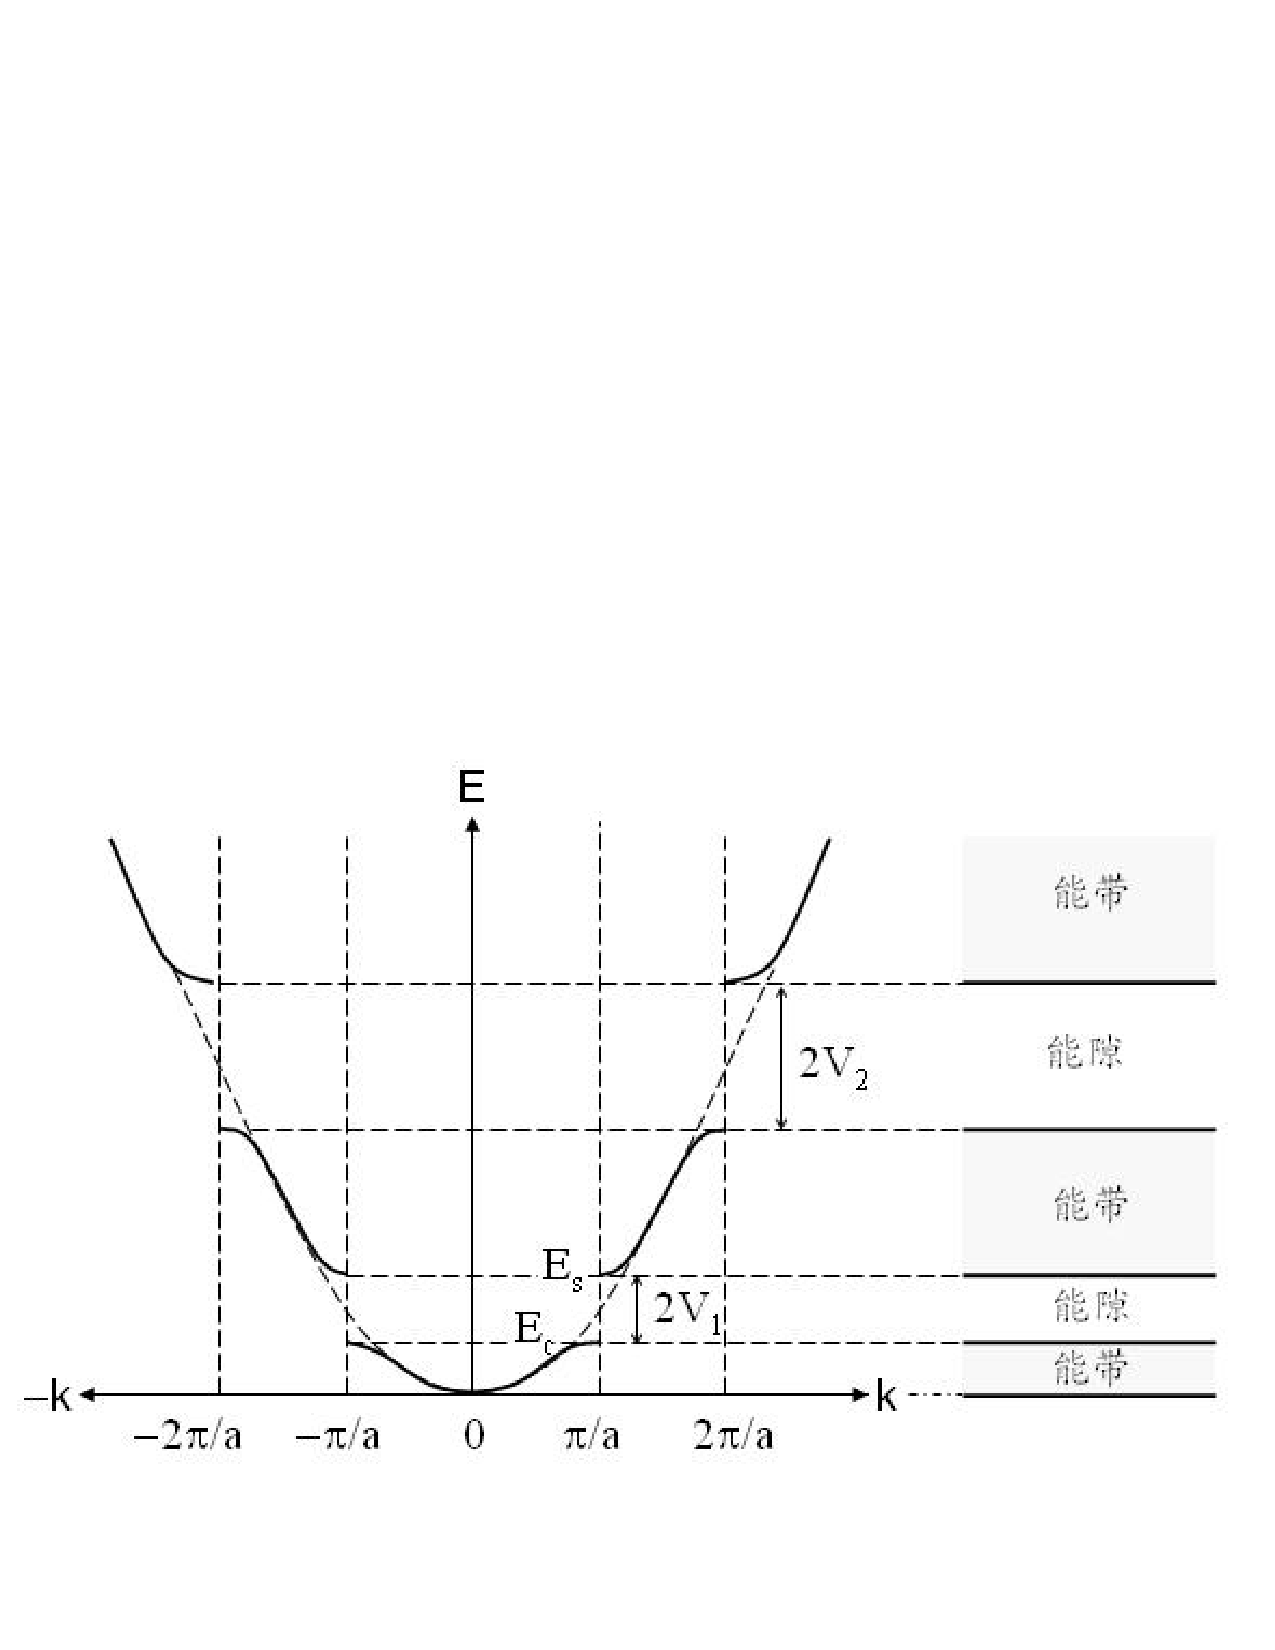
\includegraphics[height=2.1in,width=3.8in,viewport=10 90 570 380,clip]{Band_Gap.pdf}
\caption{\small \textrm{The Band-structure from free-electron gas.}}%
\label{Band-Structure-1}
\end{figure} 
}

\frame
{
\frametitle{固体能带理论}
从分子轨道到能带
\begin{figure}[h!]
\centering
\hspace*{-0.4in}
\vspace*{-0.1in}
\subfigure[\footnotesize{一维$\mathrm{H}$原子链}]{
\label{fig:Hydrogen-1D}
\includegraphics[height=0.25in,width=1.1in,viewport=70 255 570 375,clip]{Hydrogen-1D.eps}}
\subfigure[\footnotesize{$\mathrm{H}_n$分子轨道}]{
\label{fig:Hydrogen-2-n}
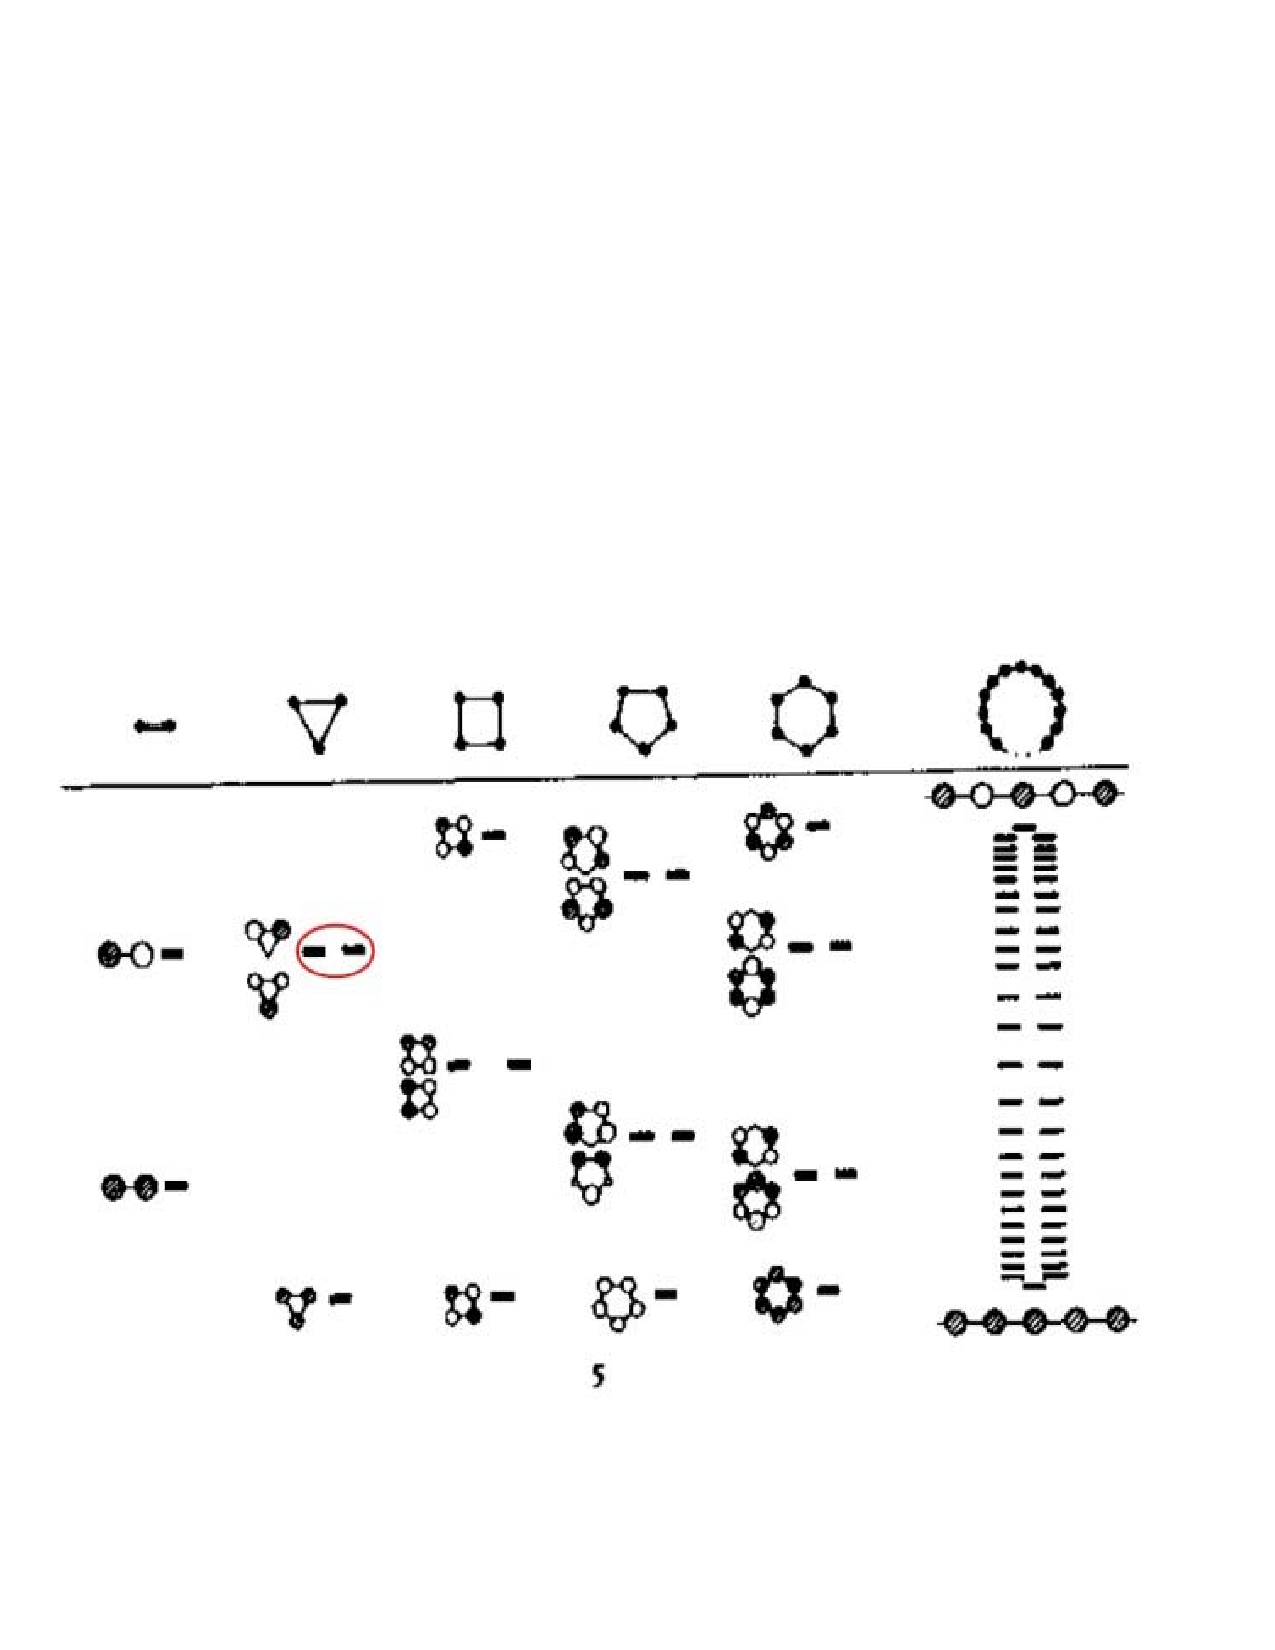
\includegraphics[height=0.8in,width=1.5in,viewport=30 140 545 480,clip]{Hydrogen-Mol-Orbital.pdf}}
\subfigure[\footnotesize{分子波函数}]{
\label{fig:Hydrogen-Psi}
\vspace*{-0.2in}
\includegraphics[height=0.5in,width=1.4in,viewport=25 218 595 440,clip]{Hydrogen-Psi.eps}}\\
\subfigure[\footnotesize{分子轨道与能带}]{
\label{fig:Hydrogen-Band-1D}
\includegraphics[height=0.6in,width=1.4in,viewport=35 215 575 450,clip]{Hydrogen-Band-1D.eps}}
\subfigure[\footnotesize{$d$轨道}]{
\label{fig:Hydrogen-d-Band-1D}
\includegraphics[height=1.0in,width=0.7in,viewport=40 45 330 535,clip]{Hydrogen-d-Band-1D.eps}}
\caption{\small \textrm{The Band-structure from Molecular-orbital.}}%
\label{Band-Structure-1}
\end{figure} 
}

\frame
{
\frametitle{周期体系的波函数}
物质的电子体系,可分为芯层分子和价层电子。芯电子能量低,受周围化学环境影响很小,基本保持原子属性;价层电子相互作用较强,对化学环境较为敏感。一般地,价电子波函数在原子间区域(\textrm{Interstitial}区)的变化平缓,在临近原子核附近区域(\textrm{Muffin-tin}球内),会出现剧烈振荡(与芯层波函数正交)。
\begin{figure}[h!]
\centering
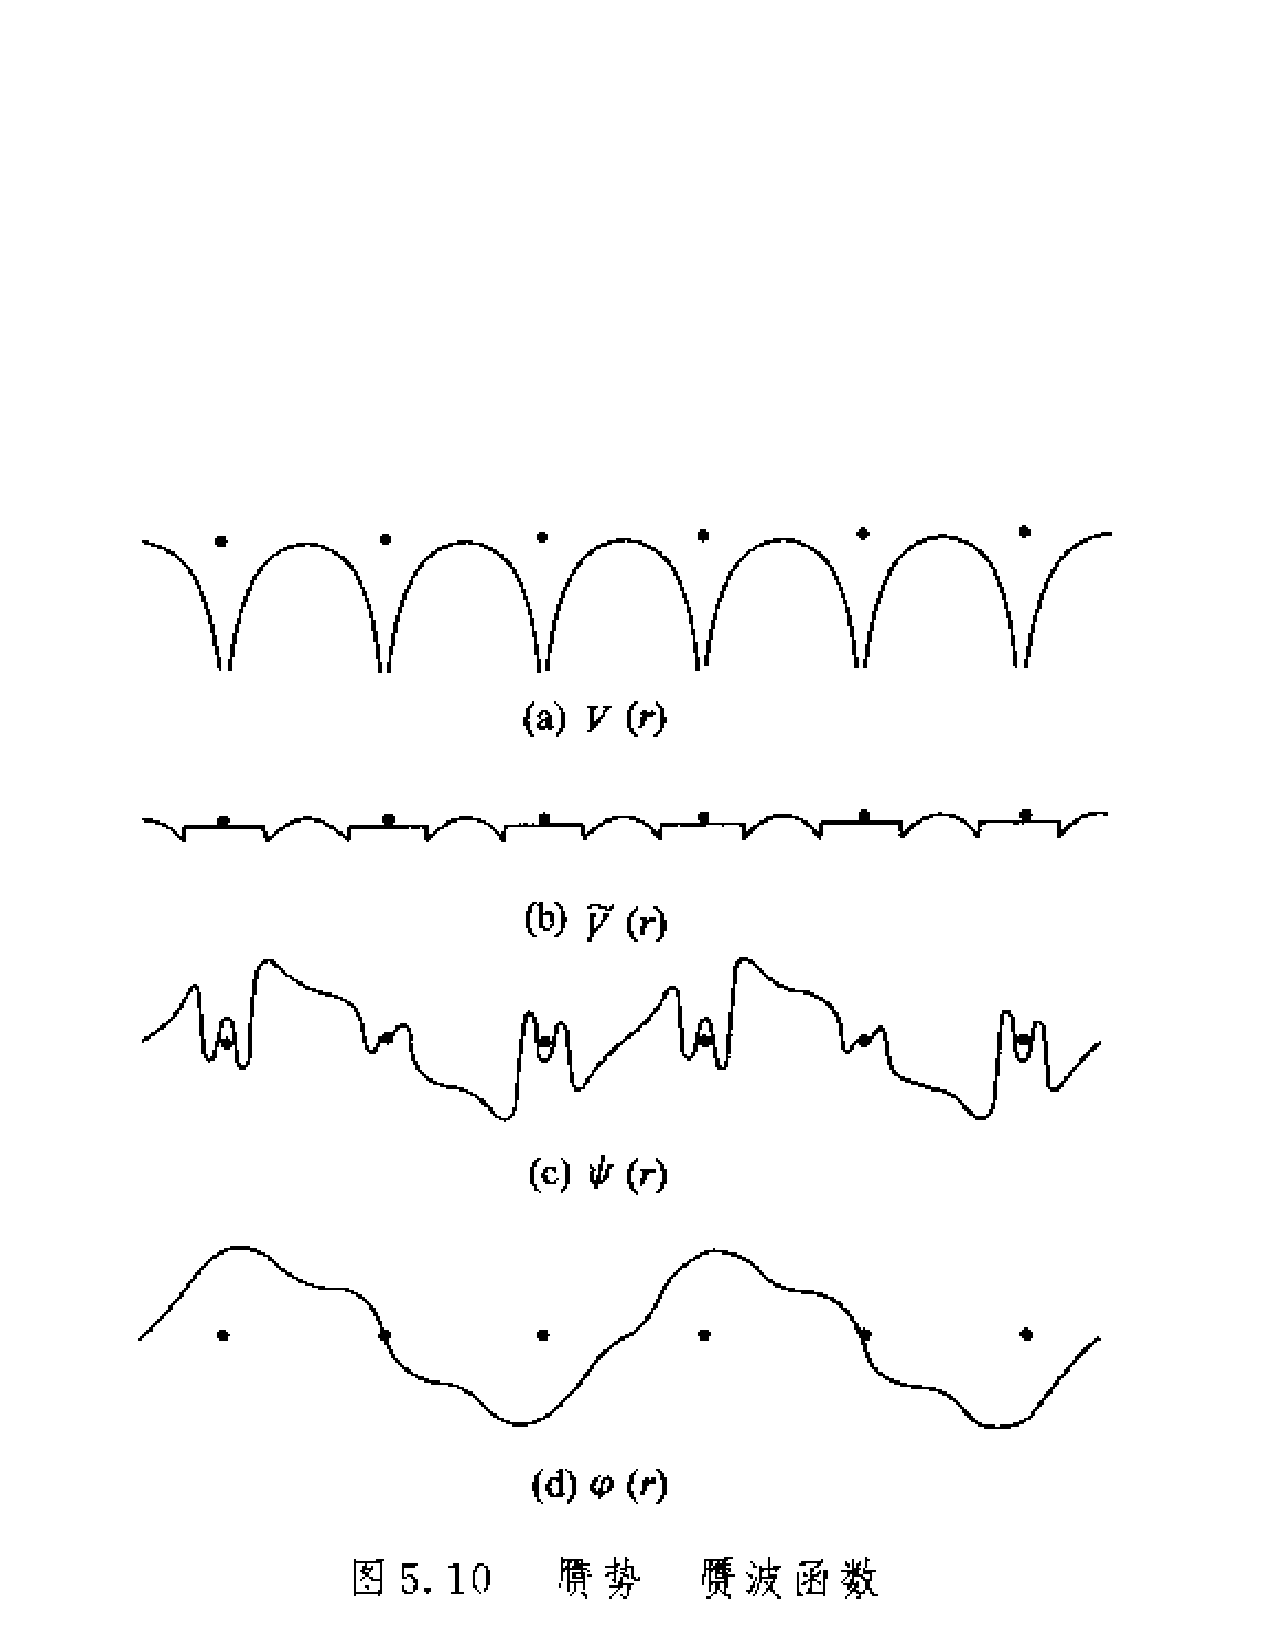
\includegraphics[height=0.8in,width=4.in,viewport=41 433 539 546,clip]{Pseudo_wave.pdf}\\
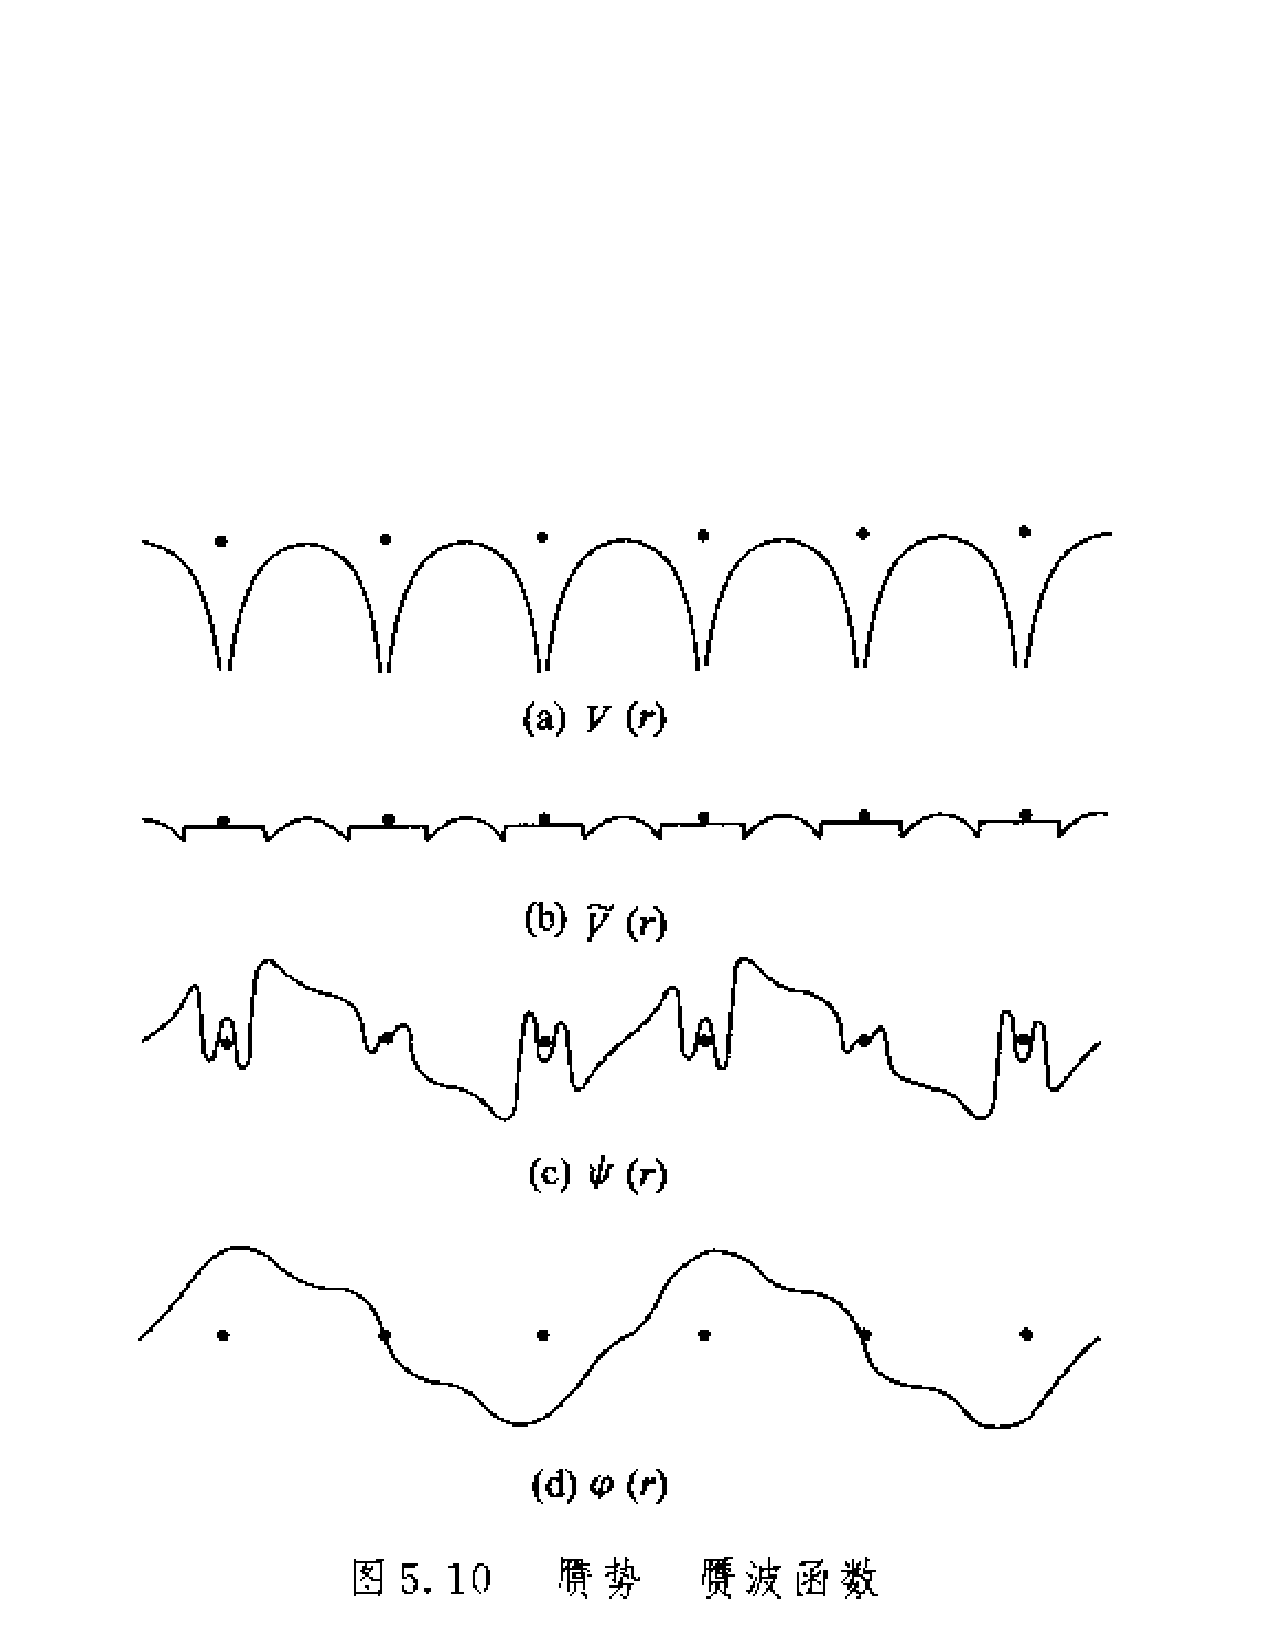
\includegraphics[height=0.8in,width=4.in,viewport=41 210 539 339,clip]{Pseudo_wave.pdf}
\caption{\small \textrm{The periodic Potential and the wave functions in crystal.}}%(与文献\cite{EPJB33-47_2003}图1对比)
\label{Potential-Wave}
\end{figure}
}

\frame
{
%\frametitle{The methods on band structure calculation}
\frametitle{固体能带计算方法}
%\vskip 10pt
%\textrm{The mainly difference of all these methods below: the basis sets and the construction of the potential}
\vskip 10pt
常用的计算方法
\begin{itemize}%[+-| alert@+>]
%\begin{enumerate}%[+-| alert@+>]
\setlength{\itemsep}{15pt}
%  \item \textrm{Plane wave and the pseudo-potential}
	\item	\textrm{平面波方法
	\item	正交平面波(The orthogonalized plane wave, OPW)和赝势(Pseudo-potential, PP)方法\upcite{Singh_Book,PRB41-7892_1990,JPCM6-8245_1994}
	\item	缀加平面波(Augmented plane wave, APW)方法
	\item	\textrm{MT}轨道(Muffin-tin orbitals, MTO)方法}
	\item	投影子缀加波\textrm{(Projector Augmented Wave, PAW)}方法\upcite{PRB50-17953_1994,PRB59-1758_1999}
\end{itemize}
  \vskip 5pt 各种方法的主要区别:所选的基函数类型不同
}

%\frame
%{
%\frametitle{}
%\begin{figure}[h!]
%\centering
%\vspace*{-10pt}
%\includegraphics[height=2.80in,width=1.70in,viewport=60 90 325 500,clip]{WIEN2k_Program_flow.eps}
%\caption{\small \textrm{Program flow in \textbf{WIEN2k}.}}%(与文献\cite{EPJB33-47_2003}图1对比)
%\label{WIEN2k_program_flow}
%\end{figure}
%}

\frame
{
%\frametitle{The methods on band structure calculation}
\frametitle{由OPW到赝势}
%\vskip 10pt
%\textrm{The mainly difference of all these methods below: the basis sets and the construction of the potential}
\begin{itemize}
\setlength{\itemsep}{5pt}
	\item 完全平面波基组,只要少数的平面波基组就可以很好地描述波函数在原子间的行为,近核的电子波函数则需要大量平面波展开。%因此完全平面波基组虽然方便,但求体系本征态对角化的矩阵非常巨大,计算变得异常耗时。
	\item 正交平面波(\textrm{Orthogonalized plane wave, OPW})方法,价电子用与芯层波函数正交的平面波展开,可以减少平面波数目
		\begin{displaymath}
			\phi_{OPW}^{\vec k+\vec G}(\vec r)=\phi_{PW}^{\vec k+\vec G}(\vec r)-\sum_{\alpha,c}\langle\varphi_c|\phi_{PW}^{\vec k+\vec G}\rangle\varphi_c(\vec r)
		\end{displaymath}
		并且势可以表示为$V^{eff}(\vec r)=V(\vec r)+V^R(\vec r)$,其中排斥部分是$$V^R(\vec r)=\sum_{\alpha,c}(\varepsilon_v-\varepsilon_c)|\varphi_c\rangle\langle\varphi_c|$$
\end{itemize}
}

\frame
{
\frametitle{赝势方法}
赝势(\textrm{Pseudo Potential, PP})方法是在正交平面波的基础上发展起来的,构造出平缓的势函数代替核的强吸引作用和芯层电子的排斥作用,用平缓的函数取代波函数近核时的震荡。
\begin{itemize}
\setlength{\itemsep}{5pt}
	\item 赝势-平面波方法,只需要少量平面波可展开赝波函数,大大提升了计算效率;但是赝波函数不能很好地反映与电子近核行为有关的性质。
	\item 赝势的构造并不唯一,考核构造赝势的两大指标:“柔软程度”\textrm{(Soft)}与“可移植性”\textrm{(transferability)}
\end{itemize}
\begin{figure}[h!]
\centering
\vspace*{-0.10in}
\includegraphics[height=1.35in,width=1.42in,viewport=154 100 562 508,clip]{Pseudo.eps}
\caption{\small \textrm{The Pseudo wave function and Pseudo potential.}}%(与文献\cite{EPJB33-47_2003}图1对比)
\label{Pseudo_Potential-Wave}
\end{figure}
}

\frame
{
\frametitle{模守恒赝势和超软赝势}
\begin{itemize}
\setlength{\itemsep}{5pt}
	\item 模守恒\textrm{(Norm-conserving)}赝势,构造赝波函数有约束条件
		\begin{displaymath}
			\int_0^{r_c}\mathrm{d}\vec r\varphi^{\ast PS}(\vec r)\varphi^{PS}(\vec r)=\int_0^{r_c}\mathrm{d}\vec r\varphi^{\ast}(\vec r)\varphi(\vec r)
		\end{displaymath}
	模守恒赝势很好地解决了赝势的可移植性问题
	\item 超软\textrm{(Ultra-soft)}赝势,解除模守恒条件,实现对第一、第二周期元素的高效计算
\end{itemize}
\begin{figure}[h!]
\centering
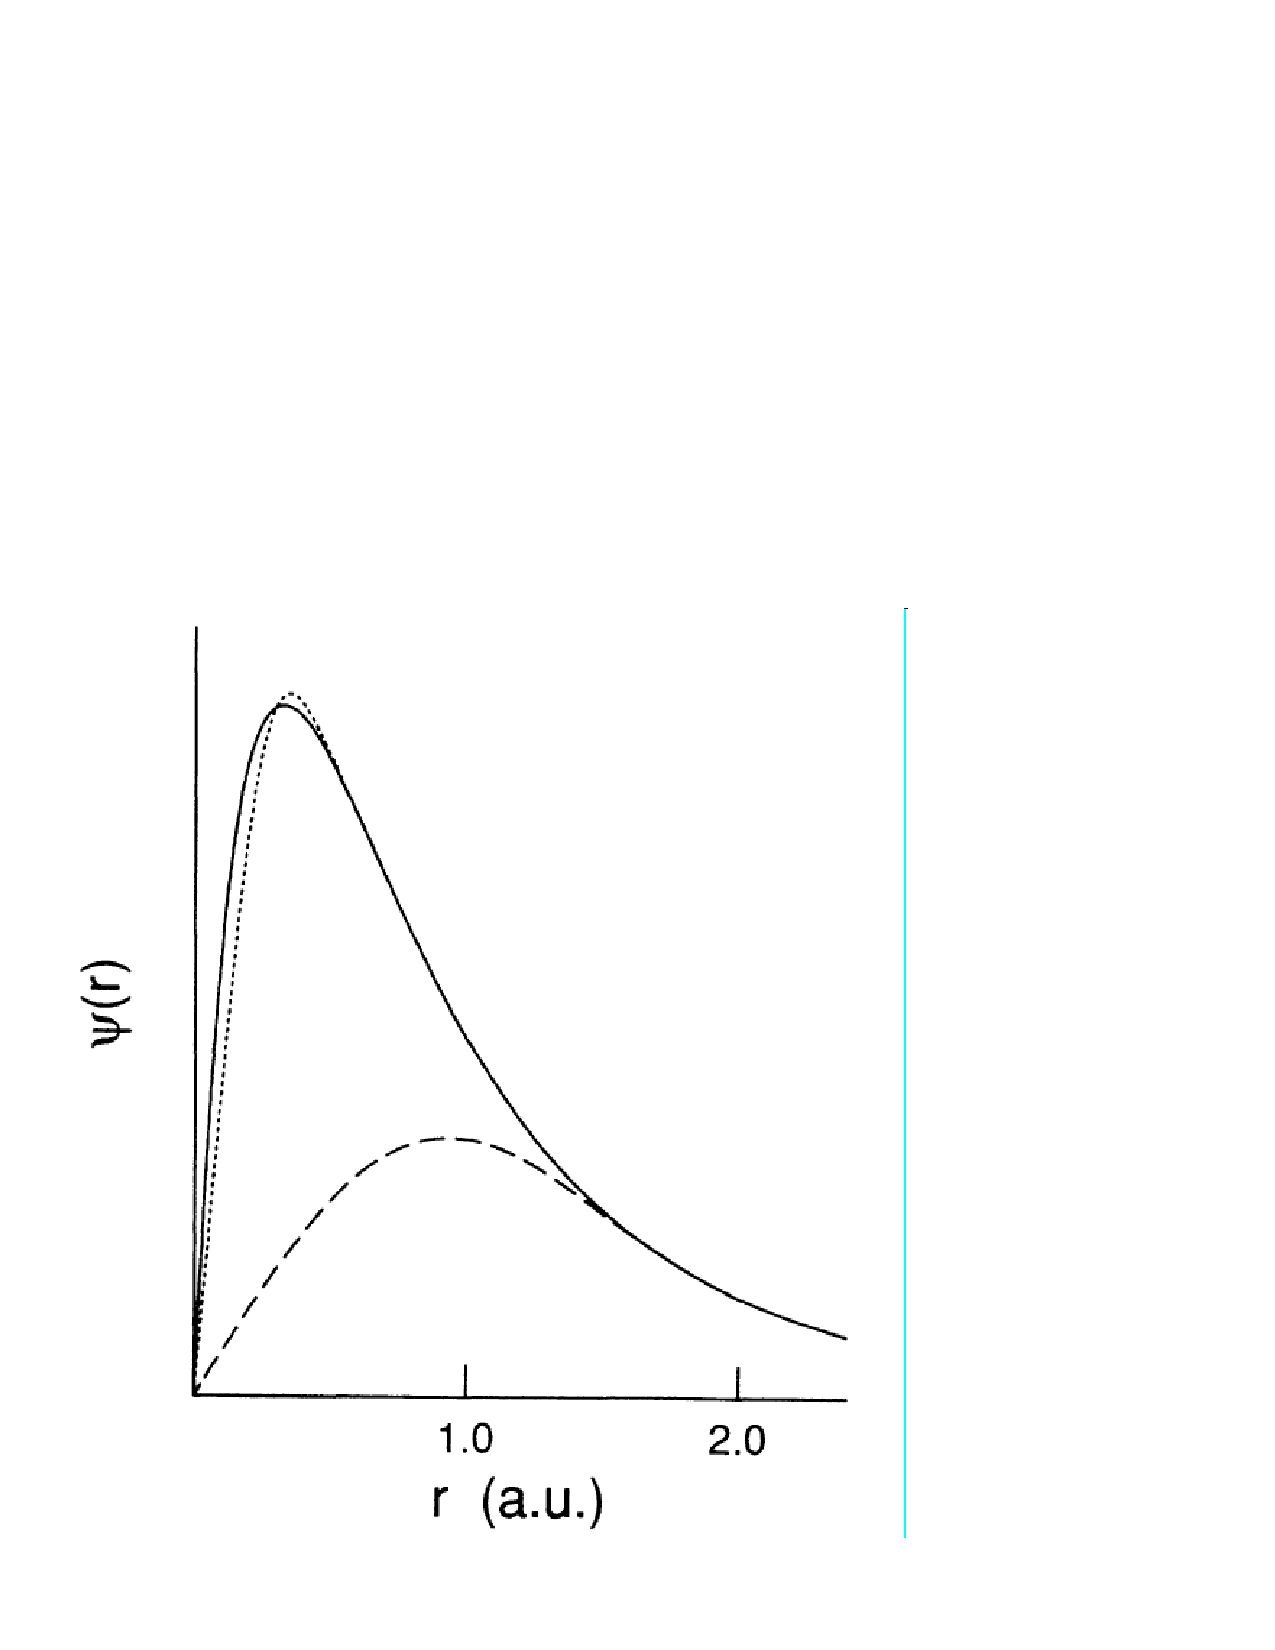
\includegraphics[height=1.35in,width=1.40in,viewport=30 55 415 500,clip]{Norm-US-wave.pdf}
\caption{\small \textrm{Oxygen 2} \textit{p} \textrm{radical wave function (solid), NC-pseudo-wave (dottde) and US-pseudo-wave (dashed).}}%(与文献\cite{EPJB33-47_2003}图1对比)
\label{Norm-US-wave}
\end{figure}
}

\frame
{
\frametitle{超软赝势}
超软赝势在平缓的局域势函数$V^L(\vec r)$和赝波函数$|\phi_{lmj}(\vec r)\rangle$的基础上,构造函数
\begin{displaymath}
	|\chi_{lmj}(\vec r)\rangle=\bigg[\varepsilon_{lj}-\dfrac12\nabla^2-V^L(\vec r)\bigg]|\phi_{lmj}(\vec r)\rangle
\end{displaymath}
在此基础上得到矩阵$\mathbf{B}_{ij}=\langle\phi_i|\chi_j\rangle$和局域函数
\begin{displaymath}
	|\beta_i\rangle=\sum_j(\mathbf{B}^{-1})_{ji}|\chi_{j}\rangle
\end{displaymath}
因此非局域赝势可以表示为
\begin{displaymath}
	V_{NL}=\dfrac{|\chi_i\rangle\langle\chi_i|}{\langle\chi_i|\chi_i\rangle}=\sum_{i,j}\mathbf{B}_{ij}|\beta_i\rangle\langle\beta_j|
\end{displaymath}
用平缓函数构造赝波函数与真实波函数的电荷密度差
\begin{displaymath}
	Q_{nm}(\vec r)=\varphi_n^{\ast}(\vec r)\varphi_m(\vec r)-\tilde\varphi_n^{\ast}(\vec r)\tilde\varphi_m(\vec r)
\end{displaymath}
}

%\section{微扰公式}       %Bookmark
\section{$\mathrm{PAW}$方法概要}
\frame
{
	\frametitle{\textrm{PAW}方法概要}
\begin{itemize}
	\item 与芯层态正交的全部价电子构成的\textrm{Hilbert}空间%,价电子彼此的正交使得波函数在\textrm{Muffin-tin}球内振荡
	\item 作\textcolor{red}{线性空间变换},全电子波函数$|\Psi\rangle$与赝波函数$|\tilde\Psi\rangle$满足:
		$$|\Psi\rangle=\mathbf{\tau|}\tilde\Psi\rangle$$
	\item 在原子核附近的$r_c$范围内,波函数用原子分波函数展开:
\begin{figure}[h!]
\centering
\vspace*{-0.20in}
\hspace*{-0.30in}
\includegraphics[height=1.32in,width=4.0in,viewport=32 233 588 437,clip]{PAW_projector.eps}
%\caption{\small \textrm{The PAW basis-sets.}}%
\label{PAW_projector}
\end{figure}
%	$$\tau=\mathbf{1}+\sum_{\mathrm R}\hat\tau_{\mathrm R}$$
%在$r_c$外$|\tilde\Psi\rangle$与$|\Psi\rangle$变换前后保持不变,因此
线性变换$\mathbf{\tau}$可表示为:
$$\mathbf{\tau}=\mathbf{1}+\sum_i(|\phi_i\rangle-|\tilde\phi_i\rangle)\langle\tilde p_i|$$
其中$|\tilde p_i\rangle$是\textrm{MT}球内的投影函数\\
$i$表示原子位置$\vec R$、原子轨道($l,m$)和能级$\epsilon_k$的指标。
\end{itemize}	
}

\frame
{
\frametitle{\textrm{PAW}方法的基本思想}
在赝波函数$|\tilde\Psi\rangle$表象下,算符期望值计算满足$$\langle A \rangle=\langle\Psi|\mathbf{A}|\Psi\rangle=\langle\tilde\Psi|\mathbf{\tau}^{\dag}\mathbf{A}\mathbf{\tau}|\tilde\Psi\rangle=\langle\tilde\Psi|\tilde{\mathrm{A}}|\tilde\Psi\rangle$$
\begin{itemize}
	\item 一般赝算符$\tilde A$表示为
		$$\tilde A=\mathbf{A}+\sum_i|\tilde p_i\rangle(\langle\phi_i|\mathbf{A}|\phi_i\rangle-\langle\tilde\phi_i|\mathbf{A}|\tilde\phi_i\rangle)\langle\tilde p_i|$$
	\item 赝重叠算符$\tilde O$表示为
		$$\tilde O=\mathbf{1}+\sum_i|\tilde p_i\rangle(\langle\phi_i|\phi_i\rangle-\langle\tilde\phi_i|\tilde\phi_i\rangle)\langle\tilde p_i|$$
\end{itemize}
}

\frame
{
\frametitle{投影函数及其特征}
上述表示中,$\tilde p_i$称为投影函数\textrm{(projector functions)}。为了确保$\tau$是线性变换,投影函数要满足一定的条件:
\begin{itemize}
	\item $$\sum_i|\tilde\phi_i\rangle\langle\tilde p_i|=1$$
	\item $$\langle\tilde p_i|\tilde\phi_j\rangle=\delta_{ij}$$
\end{itemize}
投影函数最一般的形式可以表示为:
$$\langle\tilde p_i|=\sum_j(\{\langle f_k|\tilde\phi_l\rangle\})_{ij}^{-1}\langle f_j|$$
这里$|f_j\rangle$组合成一套线性无关的函数。
}



\frame
{
\frametitle{\textrm{PAW}方法密度计算}
在\textrm{PAW}框架下,将密度算符$|\vec r\rangle\langle\vec r|$代入,可知密度表达式为
$$n(\vec r)=\tilde n(\vec r)+n^1(\vec r)-\tilde n^1(\vec r)$$
这里
$$\tilde n(\vec r)=\sum_nf_n\langle\tilde\Psi_n|\vec r\rangle\langle\vec r|\tilde\Psi_n\rangle$$ 
$$n^1(\vec r)=\sum_{n,(i,j)}f_n\langle\tilde\Psi_n|\tilde p_i\rangle\langle\phi_i|\vec r\rangle\langle\vec r|\phi_j\rangle\langle\tilde p_j|\tilde\Psi_n\rangle$$
$$\tilde n^1(\vec r)=\sum_{n,(i,j)}f_n\langle\tilde\Psi_n|\tilde p_i\rangle\langle\tilde\phi_i|\vec r\rangle\langle\vec r|\tilde\phi_j\rangle\langle\tilde p_j|\tilde\Psi_n\rangle$$
}

\frame
{
\frametitle{\textrm{PAW}方法总能量的计算}
总能量泛函
%\begin{displaymath}
%	\begin{aligned}
%		E&=\sum_nf_n\langle\Psi_n|-\dfrac12\nabla^2|\Psi_n\rangle\\
%		 &+\dfrac12\int\mathrm{d}\vec r\int\mathrm{d}\vec r^{\prime}\dfrac{(n+n^Z)(n+n^Z)}{|\vec r-\vec r^{\prime}|}+\int\mathrm{d}\vec r n\epsilon_{\mathrm{XC}}(n)
%	\end{aligned}
%\end{displaymath}
$E=\tilde E+E^1-\tilde E^1$,每一项分别表示为:
\begin{displaymath}
	\begin{aligned}
		\tilde E&=\sum_nf_n\langle\tilde\Psi_n|-\dfrac12\nabla^2|\tilde\Psi_n\rangle\\
		 &+\dfrac12\int\mathrm{d}\vec r\int\mathrm{d}\vec r^{\prime}\dfrac{(\tilde n+\hat n)(\tilde n+\hat n)}{|\vec r-\vec r^{\prime}|}+\int\mathrm{d}\vec r \tilde n\bar v+\int\mathrm{d}\vec r \tilde n\epsilon_{\mathrm{XC}}(\tilde n)
 	\end{aligned}
\end{displaymath}
\begin{displaymath}
	\begin{aligned}
		E^1&=\sum_{n,(i,j)}f_n\langle\tilde\Psi_n|\tilde p_i\rangle\langle\phi_i|-\dfrac12\nabla^2|\phi_j\rangle\langle\tilde p_j|\tilde\Psi_n\rangle\\
		 &+\dfrac12\int\mathrm{d}\vec r\int\mathrm{d}\vec r^{\prime}\dfrac{(n^1+n^Z)(n^1+n^Z)}{|\vec r-\vec r^{\prime}|}+\int\mathrm{d}\vec r n^1\epsilon_{\mathrm{XC}}(n^1)
 	\end{aligned}
\end{displaymath}
\begin{displaymath}
	\begin{aligned}
		\tilde E^1&=\sum_{n,(i,j)}f_n\langle\tilde\Psi_n|\tilde p_i\rangle\langle\tilde\phi_i|-\dfrac12\nabla^2|\tilde\phi_j\rangle\langle\tilde p_j|\tilde\Psi_n\rangle\\
		 &+\dfrac12\int\mathrm{d}\vec r\int\mathrm{d}\vec r^{\prime}\dfrac{(\tilde n^1+\hat n)(\tilde n^1+\hat n)}{|\vec r-\vec r^{\prime}|}+\int\mathrm{d}\vec r \tilde n^1\bar v+\int\mathrm{d}\vec r \tilde n^1\epsilon_{\mathrm{XC}}(\tilde n^1)
 	\end{aligned}
\end{displaymath}
}
\frame
{
	\frametitle{补偿电荷密度$\hat n$的计算}
$n^Z$表示原子核位置的点电荷密度,$\hat n$称为补偿电荷密度。\\
$\hat n$的作用:{\large\bf 使$(n^1+n^Z)$与$(\hat n^1+\hat n)$具有相同的多极矩展开},并且$\hat n=\sum\nolimits_R\hat n_R$,在每个\textrm{Muffin-tin}球内:
$$\hat n_R(r)=\sum_Lg_{RL}(r)Q_{RL}$$
其中
$$g_{RL}(r)=C_l|\vec r-\vec R|^lY_L(r-R)\mathrm{e}^{-(|\vec r-\vec R|/r_c)^2}$$
$$Q_{RL}=\int\mathrm{d}\vec r|\vec r-\vec R|^l[n^1_R(\vec r)+n^Z_R(\vec r)-\tilde n^1_R(\vec r)]Y^{\ast}_L(\vec r-\vec R)$$
如果直接计算$\hat n_R(r)$,\textrm{Gaussian}函数非常尖锐。实际计算时引入赝补偿电荷$\hat n^{\prime}$,它与$\hat n$具有相同的多极矩展开,但相应的级数$g^{\prime}_{RL}(r)$平缓得多。
}

\frame
{
	\frametitle{}
因此$\tilde E$中的静电相互作用的表达式为:
\begin{displaymath}
	\begin{aligned}
		&\dfrac12\int\mathrm{d}\vec r\int\mathrm{d}\vec r^{\prime}\dfrac{(\tilde n+\hat n)(\tilde n+\hat n)}{|\vec r-\vec r^{\prime}|}\\
	=&\dfrac12\int\mathrm{d}\vec r\int\mathrm{d}\vec r^{\prime}\dfrac{(\tilde n+\hat n^{\prime})(\tilde n+\hat n^{\prime})}{|\vec r-\vec r^{\prime}|}\\
		&+\int\mathrm{d}\vec r\int\mathrm{d}\vec r^{\prime}\tilde n(\vec r)\dfrac{\hat n(\vec r^{\prime})-\hat n^{\prime}(\vec r^{\prime})}{|\vec r-\vec r^{\prime}|}\\
		&+\sum_{\vec R,\vec R^{\prime}}\dfrac12\int\mathrm{d}\vec r\int\mathrm{d}\vec r^{\prime}\dfrac{\hat n_R(\vec r)\hat n_{R^{\prime}}(\vec r^{\prime})-\hat n^{\prime}_R(\vec r)\hat n^{\prime}_{R^{\prime}}(\vec r^{\prime})}{|\vec r-\vec r^{\prime}|}
	\end{aligned}
\end{displaymath}
}

%\section{PAW基组}
\frame
{
	\frametitle{PAW方法的Hamilton算符}
%重叠算符:
%$$\tilde O=1+\sum_{i,j}|\tilde p_i\rangle[\langle\phi_i|\phi_j\rangle-\langle\tilde\phi_i|\tilde\phi_j\rangle]\langle\tilde p_j|$$
\textrm{Hamiliton}算符
\begin{itemize}
	\item 动能算符:
		$$\tilde T=-\dfrac12\nabla^2+\sum_{i,j}|\tilde p_i\rangle[\langle\phi_i|-\dfrac12\nabla^2|\phi_j\rangle-\langle\tilde\phi_i|-\dfrac12\nabla^2|\tilde\phi_j\rangle]\langle\tilde p_j|$$
	\item 完全势\textrm{(full-potential)}算符:
$$v(\vec r)=\tilde v(\vec r)+v^1(\vec r)-\tilde v^1(\vec r)$$
	\item \textrm{Hamilton}算符:
		$$\hspace*{-10pt}\tilde H=-\dfrac12\nabla^2+\tilde v+\sum_{i,j}|\tilde p_i\rangle[\langle\phi_i|-\dfrac12\nabla^2+v^1|\phi_j\rangle-\langle\tilde\phi_i|-\dfrac12\nabla^2+\tilde v^1|\tilde\phi_j\rangle]\langle\tilde p_j|$$
\end{itemize}
}

\frame
{
	\frametitle{分波函数$\phi_i$的构造}
	\begin{itemize}
		\item 全电子分波函数由方程:
			$$\biggl(\dfrac12\nabla^2+v_{at}-\epsilon_i^1\biggr)|\phi_i\rangle=0$$
			计算得到
		\item 赝势分波函数由方程:
			$$\biggl(\dfrac12\nabla^2+w_{i}(\vec r)-\epsilon_i^1\biggr)|\tilde\phi_i\rangle=0$$
			计算得到。\\
			这里$w_i(\vec r)=\tilde v_{at}(\vec r)+c_ik(\vec r)$,由赝势$\tilde v_{at}(\vec r)$确定。
%		\item 赝势$\tilde v_{at}(\vec r)$的确定:对不含\textit{d}电子体系与过渡元素体系采用不同的形式。
		\end{itemize}
}

\frame
{
	\frametitle{投影函数$\tilde p_i$的构造}
	\begin{itemize}
		\item $\tilde p_i$由递推方式得到,初始的$\tilde p_i$的生成:
			$$|\tilde p_i\rangle=\biggl(\dfrac12\nabla^2+\tilde v_{at}-\epsilon_i^1\biggr)|\tilde\phi_i\rangle$$
		\item 根据正交关系$\langle\tilde p_i|\tilde\phi_j\rangle=\delta_{ij}$有:
			$$|\tilde p_i\rangle=|\tilde p_i\rangle-\sum_{j=1}^{i-1}|\tilde p_j\rangle\langle\tilde\phi_j|\tilde p_i\rangle$$
%		为确保分波函数与投影函数正交:
%			$$|\phi_i\rangle=|\phi_i\rangle-\sum_{j=1}^{i-1}|\phi_j\rangle\langle\tilde p_j|\tilde\phi_i\rangle$$
%			$$|\tilde\phi_i\rangle=|\tilde\phi_i\rangle-\sum_{j=1}^{i-1}|\tilde\phi_j\rangle\langle p_j|\tilde\phi_i\rangle$$
		\end{itemize}
}

%\section{PAW方法在VASP程序中的实现}
\frame
{
\frametitle{电荷密度的重新分解}
\textrm{PAW}方法提出后有很长一段时间没有能够得到广泛应用,直到\textrm{G. Kresse}等将\textrm{Bl\"ochl}的原始方案中电荷密度计算方案重新组合后,明确了\textrm{PAW}方法与\textrm{USPP}方法的内在联系。
\begin{itemize}
	\item 芯层电荷与核电荷构成离子实电荷:$n_{Zc}=n_Z+n_c$
	\item 赝离子实电荷的构造$$\int_{\Omega_c}n_{Zc}(\vec r)\mathrm{d}^3\vec r=\int_{\Omega_c}\tilde n_{Zc}(\vec r)\mathrm{d}^3\vec r$$
\end{itemize}
在此基础上,\textrm{Bl\"ochl}方案中的电荷可以分解为:
\begin{displaymath}
	\begin{aligned}
		n_T=n+n_{Zc}\equiv&\underbrace{(\tilde n+\hat n+\tilde n_{Zc})}\\
				 		&\quad\qquad\tilde n_T\\
				  &+\underbrace{(n^1+\hat n+n_{Zc})}-\underbrace{(\tilde n^1+\hat n+\tilde n_{Zc})}\\
				                  &\quad\qquad n_T^1\qquad\qquad\qquad\tilde n_T^1
	\end{aligned}
\end{displaymath}
\textcolor{red}{注意}:\textrm{G. Kresse}方案中补偿电荷$\hat n$局域在每个缀加球内。
}

\frame
{
\frametitle{Hartree势的分解}
\begin{displaymath}
	\begin{aligned}
		\dfrac12(n_T)(n_T)=&\dfrac12(\tilde n_T)(\tilde n_T)+(n_T^1-\tilde n_T^1)(\tilde n_T)\\
				&+\dfrac12(n_T^1-\tilde n_T^1)(n_T^1-\tilde n_T)
	\end{aligned}
\end{displaymath}
这里$$(a)(b)=\int\mathrm{d}\vec r\mathrm{d}\vec r^{\prime}\dfrac{a(\vec r)b(\vec r)}{|\vec r-\vec r^{\prime}|}$$
\textcolor{red}{近似}:$\tilde n_T$用$\tilde n_T^1$替换:
\begin{displaymath}
	\dfrac12(n_T)(n_T)=\dfrac12(\tilde n_T)(\tilde n_T)-\dfrac12\overline{(n_T^1(\tilde n_T^1)}+\dfrac12\overline{(n_T^1)(n_T^1)}
\end{displaymath}
}

\frame
{
\frametitle{交换-相关能泛函的处理}
由于交换-相关能泛函是非线性的,\textrm{G. Kresse}方案中电荷密度分解为
\begin{displaymath}
	n_c+n=(\tilde n+\hat n+\tilde n_c)+(n^1+n_c)-(\tilde n^1+\hat n+\tilde n_c)
\end{displaymath}
原始的\textrm{Bl\"ochl}方案中电荷分解为
\begin{displaymath}
	n_c+n=(\tilde n)+(n^1+n_c)-(\tilde n^1)
\end{displaymath}
\textcolor{blue}{两种不同的电荷密度分解方案根源}:\\\textrm{G. Kresse}方案中赝离子实电荷$\tilde n_{Zc}$与\textrm{Bl\"ochl}方案中$\tilde n_c$的约束条件不同!
\begin{displaymath}
	E_{\mathrm{XC}}[\tilde n+\hat n+\tilde n_c]+\overline{E_{\mathrm{XC}}[n^1+n_c]}-\overline{E_{\mathrm{XC}}[\tilde n^1+\hat n+\tilde n_c]}
\end{displaymath}
}

\frame
{
	\frametitle{补充电荷的构造}
	根据约束条件
	\begin{displaymath}
		\int_{\Omega_c}(n^1-\tilde n^1-\hat n)|\vec r-\vec R|^lY_{lm}^{\ast}(\widehat{\vec r-\vec R})\mathrm{\vec r}=0
	\end{displaymath}
	定义电荷密度差
	\begin{displaymath}
		Q_{ij}(\vec r)=\phi_i^{\ast}(\vec r)\phi_j(\vec r)-\tilde\phi_i^{\ast}(\vec r)\tilde\phi_j(\vec r)
	\end{displaymath}
	电荷密度差的多极矩为
	\begin{displaymath}
		q_{ij}^L(\vec r)=\int_{\Omega_c}Q_{ij}(\vec r)|\vec r-\vec R|^lY_{lm}^{\ast}(\widehat{\vec r-\vec R})\mathrm{\vec r}
	\end{displaymath}
	因此,补充电荷的计算为:
	\begin{displaymath}
		\begin{aligned}
			\hat n=\sum_{(i,j),L}\sum_n f_n\langle\tilde\Psi_n|\tilde p_i\rangle\langle\tilde p_j|\Psi_n\rangle\hat Q_{ij}^L(\vec r)\\
			\hat Q_{ij}^L(\vec r)=q_{ij}^Lg_l(|\vec r-\vec R|)Y_{lm}(\widehat{\vec r-\vec R})
		\end{aligned}
	\end{displaymath}
}


\frame
{
	\frametitle{重叠矩阵和Hamiltonian的构造}
重叠矩阵
	\begin{displaymath}
		\langle\tilde\Psi_n|\mathbf{S}|\tilde\Psi_m\rangle=\delta_{nm}
	\end{displaymath}
	其中重叠矩阵$$S[\{\mathbf{R}\}]=1+\sum_i|\tilde p_i\rangle q_{ij}\langle\tilde p_j|$$
	而$$q_{ij}=\langle\phi_i|\phi_j\rangle-\langle\tilde\phi_i|\tilde\phi_j\rangle$$
	\textrm{Hamiltonian}的计算
	\begin{displaymath}
		H[\rho,\{\mathbf{R}\}]=-\dfrac12\nabla^2+\tilde v_{eff}+\sum_{(i,j)}|\tilde p_i\rangle(\hat D_{ij}+D_{ij}^1-\tilde D_{ij}^1)\langle\tilde p_j|	
	\end{displaymath}
	$$\tilde v_{eff}=v_H[\tilde n+\hat n+\tilde n_{Zc}]+v_{\mathrm{XC}}[\tilde n+\hat n+\tilde n_{Zc}]$$
}

\frame
{
	\frametitle{重叠矩阵和Hamiltonian的构造}
	$$\hat D_{ij}=\dfrac{\partial\tilde E}{\partial\rho_{ij}}=\int\dfrac{\delta\tilde E}{\delta\hat n(\vec  r)}\dfrac{\partial\hat n(\vec r)}{\partial\rho_{ij}}\mathrm{d}\vec r=\sum_{L}\int\tilde v_{eff}\hat Q_{ij}^L(\vec r)\mathrm{d}\vec r$$
	$$D_{ij}^1=\dfrac{\partial E^1}{\partial\rho_{ij}}=\langle\phi_i|-\dfrac12\nabla^2+v_{eff}^1|\phi_j\rangle$$
	其中$$v_{eff}^1[n^1]=v_H[n^1+n_{Zc}]+v_{\mathrm{XC}}[n^1+n_c]$$
	$$\tilde D_{ij}^1=\dfrac{\partial\tilde E^1}{\partial\rho_{ij}}=\langle\tilde\phi_i|-\dfrac12\nabla^2+\tilde v_{eff}^1|\tilde\phi_j\rangle+\sum_L\int_{\Omega_r}\mathrm{d}\vec r\tilde v_{eff}^1(\vec r)\hat Q_{ij}^L$$
	其中$$\tilde v_{eff}^1[\tilde n^1]=v_H[\tilde n^1+\hat n+\tilde n_{Zc}]+v_{\mathrm{XC}}[\tilde n^1+\hat n+\tilde n_c]$$
}

\frame
{
	\frametitle{\textrm{PAW}原子数据集}
\textrm{PAW}原子数据集是在原子核附近$r_c$范围内将波函数用原子分波\\展开所需信息的统称,是\textrm{PAW}计算的基础。

\textrm{PAW}原子数据集主要包括
	\begin{itemize}
		\item 分波信息:原子分波$\phi_i$、赝分波$\tilde\phi_i$和投影子波函数$p_i$
		\item 密度信息:$r_c$内的电荷密度$n^1$、赝电荷密度$\tilde n^1$和补充电荷$\hat n$
		\item 赝势信息:局域赝势$\tilde v_{loc}(\vec r)$
	\end{itemize}
	与赝势方法相似,一套原子数据集将用于各种化学环境下的\textrm{PAW}\\计算,即要求原子数据集有良好的可移植性;与赝势方法不同之\\处在于\textrm{PAW}原子集中除了赝原子的信息,还包含了真实原子的信\\息。
}

%\frame
%{
%\frametitle{\textrm{WIEN2k}程序中基函数的选择}
%\vskip 10pt
%\begin{itemize}
%\setlength{\itemsep}{15pt}
%	\item 对\textit{s}态、\textit{p}态价电子轨道用\textrm{LAPW}基组展开
%	\item 对一般平面波基函数展开收敛缓慢的轨道(如过渡金属的3\textit{d}态波函数)或\textrm{MT}球半径特别小的体系用\textrm{APW+lo}基组展开
%	\item 对半芯层轨道用\textrm{LAPW-LO}基组展开
%\end{itemize}
%这样搭配选择基组,可以同时较好地处理价态和半芯态。
%}
%\frame
%{
%\frametitle{LDA近似下的总能量表达式}
%\begin{itemize}
%	\item 间隙区的电荷密度用平面波展开:\footnotesize{$\rho(\vec r)=\sum\limits_{\vec G}\rho(\vec G)\mathrm{e}^{i\vec G\cdot\vec r}$}
%	\item 在\textrm{MT}球内,电荷密度用球谐函数展开,在动量空间中的展开形式为:\footnotesize{$\bar\rho_{lm}(r_{\nu})=4\pi i^l\sum\limits_{\vec G}\rho(\vec G)\mathrm{e}^{i\vec G\cdot\vec r_{\nu}}j_l(\vec G\cdot\vec r_{\nu})Y_{lm}^{\ast}(\vec G)$}
%\end{itemize}
%\textrm{LDA}近似下,\footnotesize{$$E_{XC}[\rho]\approx\int_{\Omega}\rho(\vec r)\varepsilon_{XC}(\vec r)\textrm{d}\vec r$$}
%因此\textrm{WS}原胞内的晶体总能量可以写成:
%{\footnotesize
%\begin{displaymath}
%  \begin{split}
%\hskip -10pt	  E=&\sum_i\varepsilon_i-\Omega\sum_{\vec G}\rho(\vec G)\tilde V^{\ast}(\vec G)-\frac12\sum_{\nu}\dfrac{Z_{\nu}}{R_{\nu}}[Z_{\nu}-Q_{\nu}+R_{\nu}S_0(R_{\nu})]\\
%    &-\sum_{\nu}\sum_{lm}\int_0^{R_{\nu}}\mathrm{d}rr^2\left[\rho_{lm}(r_{\nu})\left(\tilde V_{lm}^{\ast}(r_{\nu})+\dfrac{\sqrt{4\pi}}{2r_{\nu}}Z_{\nu}\delta_{l0}\right)-\bar\rho_{lm}(\vec r_{\nu})\bar V_{lm}^{\ast}(\vec r_{\nu})\right]
%  \end{split}
%  \label{eq:solid-83}
%\end{displaymath}}
%这里$\tilde V(\vec r)$和$\bar V_{lm}(\vec r)$根据都按下式计算:
%\footnotesize{$$\tilde V(\vec r)=\frac12V_C(\vec r)-\varepsilon_{XC}(\vec r)+\mu_{XC}(\vec r)$$}
%}

%\frame
%{
%\frametitle{}
%\begin{figure}[h!]
%\centering
%\hspace*{-10pt}
%\includegraphics[height=1.72in,width=4.2in,viewport=30 165 550 375,clip]{WIEN2k_Data_flow.eps}
%\caption{\small \textrm{Data flow during a SCF cycle (programX.def, case.struct, case.inX, case.outputX and optional files are omitted).}}%(与文献\cite{EPJB33-47_2003}图1对比)
%\label{WIEN2k_Data_flow}
%\end{figure}
%}

%\frame
%{
%\frametitle{PAW方法基本思想}
%$\hat\tau_{\mathrm R}$的定义是在\textrm{Muffin-tin}球区,$\hat\tau_{\mathrm R}$使得赝原子波函数$\tilde\phi_i$与全原子波函数$\phi_i$之间的变换关系满足:
%$$|\phi_i\rangle=(1+\hat\tau_{\mathrm R})|\tilde\phi_i\rangle$$

%在每个\textrm{Muffin-tin}球内,体系的赝波函数用赝原子波函数展开:
%$$|\tilde\Psi\rangle=\sum_i|\tilde\phi_i\rangle c_i$$
%由于$|\phi_i\rangle=\tau|\tilde\phi_i\rangle$,因此\textrm{Muffin-tin}球内全电子波函数可以表示为:
%$$|\Psi\rangle=\tau|\tilde\Psi\rangle=\sum_i|\phi_i\rangle c_i$$
%因此,全电子波函数可以表示为:
%$$|\Psi\rangle=|\tilde\Psi\rangle-\sum_i|\tilde\phi_i\rangle c_i+\sum_i|\phi_i\rangle c_i$$
%}

%\frame
%{
%\frametitle{投影函数及其特征}
%为了确保$\tau$是线性变换,它必须是赝波函数$\tilde\Psi$的线性函数。因此系数$c_i$满足:
%$$c_i=\langle\tilde p_i|\tilde\Psi\rangle$$
%这里$\tilde p_i$称为投影函数\textrm{(projector functions)}。
%投影函数要满足的条件:
%\begin{itemize}
%	\item $$\sum_i|\tilde\phi_i\rangle\langle\tilde p_i|=1$$
%	\item $$\langle\tilde p_i|\tilde\phi_j\rangle=\delta_{ij}$$
%\end{itemize}
%投影函数最一般的形式可以表示为:
%$$\langle\tilde p_i|=\sum_j(\{\langle f_k|\tilde\phi_l\rangle\})_{ij}^{-1}\langle f_j|$$
%这里$|f_j\rangle$组合成一套线性无关的函数。
%}

%\frame
%{
%\frametitle{}
%线性变换算符可以表示为:
%$$\tau=1+\sum_i(|\phi_i\rangle-|\tilde\phi_i\rangle)\langle\tilde p_i|$$
%因此,全电子波函数的表达式为:
%$$|\Psi\rangle=|\tilde\Psi\rangle+\sum_i(|\phi_i\rangle-|\tilde\phi_i\rangle)\langle\tilde p_i|\tilde\Psi\rangle$$

%对于芯层态$|\Psi^c\rangle$,处理与价层态类似:
%$$|\Psi^c\rangle=|\tilde\Psi^c\rangle+|\phi^c\rangle-|\tilde\phi^c\rangle$$
%但芯层态不需要定义相应的投影函数,本质上是冻芯近似的处理方式。
%}

%\frame
%{
%\frametitle{PAW方法的算符和密度表示}
%因为引入变换算符$\tau$,波函数由\textrm{Schr\"odinger}表象变为\textrm{Heisenberg}表象。因此在赝波函数构成的\textrm{Hilbert}空间内,算符的变换满足:
%\begin{displaymath}
%\begin{aligned}
%	\tilde A &=\tau^{\dag}A\tau \\
%			&=A+\sum_{i,j}|\tilde p_i\rangle(\langle\phi_i|A|\phi_j\rangle-\langle\tilde\phi_i|A|\tilde\phi_j\rangle)\langle\tilde p_j|
%\end{aligned}
%\end{displaymath}
%由此,可以得到电荷密度的表达式为:
%$$n(\vec r)=\tilde n(\vec r)+n^1(\vec r)-\tilde n^1(\vec r)$$
%\footnotesize{
%这里
%$$\tilde n(\vec r)=\sum_nf_n\langle\tilde\Psi_n|\vec r\rangle\langle\vec r|\tilde\Psi_n\rangle$$
%$$n^1(\vec r)=\sum_{n,(i,j)}f_n\langle\tilde\Psi_n|\tilde p_i\rangle\langle\phi_i|\vec r\rangle\langle\vec r|\phi_j\rangle\langle\tilde p_j|\tilde\Psi_n\rangle$$
%$$\tilde n^1(\vec r)=\sum_{n,(i,j)}f_n\langle\tilde\Psi_n|\tilde p_i\rangle\langle\tilde\phi_i|\vec r\rangle\langle\vec r|\tilde\phi_j\rangle\langle\tilde p_j|\tilde\Psi_n\rangle$$
%}}

%\frame
%{
%	\frametitle{总能量的表示}
%总能量泛函
%\begin{displaymath}
%	\begin{aligned}
%		E&=\sum_nf_n\langle\Psi_n|-\dfrac12\nabla^2|\Psi_n\rangle\\
%		 &+\dfrac12\int\mathrm{d}\vec r\int\mathrm{d}\vec r^{\prime}\dfrac{(n+n^Z)(n+n^Z)}{|\vec r-\vec r^{\prime}|}+\int\mathrm{d}\vec r n\epsilon_{\mathrm{XC}}(n)
%	\end{aligned}
%\end{displaymath}
%与密度表达式类似,$E=\tilde E+E^1-\tilde E^1$,每一项分别表示为:
%\footnotesize{
%\begin{displaymath}
%	\begin{aligned}
%		\tilde E&=\sum_nf_n\langle\tilde\Psi_n|-\dfrac12\nabla^2|\tilde\Psi_n\rangle\\
%		 &+\dfrac12\int\mathrm{d}\vec r\int\mathrm{d}\vec r^{\prime}\dfrac{(\tilde n+\hat n)(\tilde n+\hat n)}{|\vec r-\vec r^{\prime}|}+\int\mathrm{d}\vec r \tilde n\bar v+\int\mathrm{d}\vec r \tilde n\epsilon_{\mathrm{XC}}(\tilde n)
%	\end{aligned}
%\end{displaymath}
%\begin{displaymath}
%	\begin{aligned}
%		E^1&=\sum_{n,(i,j)}f_n\langle\tilde\Psi_n|\tilde p_i\rangle\langle\phi_i-\dfrac12\nabla^2|\phi_j\rangle\tilde p_j\tilde\Psi_n\rangle\\
%		 &+\dfrac12\int\mathrm{d}\vec r\int\mathrm{d}\vec r^{\prime}\dfrac{(n^1+n^Z)(n^1+n^Z)}{|\vec r-\vec r^{\prime}|}+\int\mathrm{d}\vec r n^1\epsilon_{\mathrm{XC}}(n^1)
%	\end{aligned}
%\end{displaymath}
%\begin{displaymath}
%	\begin{aligned}
%		\tilde E^1&=\sum_{n,(i,j)}f_n\langle\tilde\Psi_n|\tilde p_i\rangle\langle\tilde\phi_i-\dfrac12\nabla^2|\tilde\phi_j\rangle\tilde p_j\tilde\Psi_n\rangle\\
%		 &+\dfrac12\int\mathrm{d}\vec r\int\mathrm{d}\vec r^{\prime}\dfrac{(\tilde n^1+\hat n)(\tilde n^1+\hat n)}{|\vec r-\vec r^{\prime}|}+\int\mathrm{d}\vec r \tilde n^1\bar v+\int\mathrm{d}\vec r \hat n^1\epsilon_{\mathrm{XC}}(\hat n^1)
%	\end{aligned}
%\end{displaymath}
%}}

%\frame
%{
%	\frametitle{补偿电荷密度$\hat n$的计算}
%$n^Z$表示原子核位置的点电荷密度,$\hat n$称为补偿电荷密度。\\
%$\hat n$的作用:\large{\bf 使$(n^1+n^Z)$与$(\hat n^1+\hat n)$具有相同的多极矩展开},并且$\hat n=\sum\nolimits_R\hat n_R$,在每个\textrm{Muffin-tin}球内:
%$$\hat n_R(r)=\sum_Lg_{RL}(r)Q_{RL}$$
%其中
%$$g_{RL}(r)=C_l|\vec r-\vec R|^lY_L(r-R)\mathrm{e}^{-(|\vec r-\vec R|/r_c)^2}$$
%$$Q_{RL}=\int\mathrm{d}\vec r|\vec r-\vec R|^l[n^1_R(\vec r)+n^Z_R(\vec r)-\tilde n^1_R(\vec r)]Y^{\ast}_L(\vec r-\vec R)$$
%如果直接计算$\hat n_R(r)$,\textrm{Gaussian}函数非常尖锐。实际计算时引入赝补偿电荷$\hat n^{\prime}$,它与$\hat n$具有相同的多极矩展开,但相应的级数$g^{\prime}_{RL}(r)$平缓得多。
%}

%\frame
%{
%	\frametitle{}
%因此$\tilde E$中的静电相互作用的表达式为:
%\begin{displaymath}
%	\begin{aligned}
%		&\dfrac12\int\mathrm{d}\vec r\int\mathrm{d}\vec r^{\prime}\dfrac{(\tilde n+\hat n)(\tilde n+\hat n)}{|\vec r-\vec r^{\prime}|}\\
%	=&\dfrac12\int\mathrm{d}\vec r\int\mathrm{d}\vec r^{\prime}\dfrac{(\tilde n+\hat n^{\prime})(\tilde n+\hat n^{\prime})}{|\vec r-\vec r^{\prime}|}\\
%		&+\int\mathrm{d}\vec r\int\mathrm{d}\vec r^{\prime}\tilde n(\vec r)\dfrac{\hat n(\vec r^{\prime})-\hat n^{\prime}(\vec r^{\prime})}{|\vec r-\vec r^{\prime}|}\\
%		&+\sum_{\vec R,\vec R^{\prime}}\dfrac12\int\mathrm{d}\vec r\int\mathrm{d}\vec r^{\prime}\dfrac{\hat n_R(\vec r)\hat n_{R^{\prime}}(\vec r^{\prime})-\hat n^{\prime}_R(\vec r)\hat n^{\prime}_{R^{\prime}}(\vec r^{\prime})}{|\vec r-\vec r^{\prime}|}
%	\end{aligned}
%\end{displaymath}
%}

%\frame
%{
%	\frametitle{PAW方法的重叠算符和Hamilton算符}
%重叠算符:
%$$\tilde O=1+\sum_{i,j}|\tilde p_i\rangle[\langle\phi_i|\phi_j\rangle-\langle\tilde\phi_i|\tilde\phi_j\rangle]\langle\tilde p_j|$$
%\textrm{Hamiliton}算符
%\begin{itemize}
%	\item 动能算符:
%		$$\tilde T=-\dfrac12\nabla^2+\sum_{i,j}|\tilde p_i\rangle[\langle\phi_i|-\dfrac12\nabla^2|\phi_j\rangle-\langle\tilde\phi_i|-\dfrac12\nabla^2|\tilde\phi_j\rangle]\langle\tilde p_j|$$
%	\item 完全势\textrm{(full-potential)}算符:
%$$v(\vec r)=\tilde v(\vec r)+v^1(\vec r)-\tilde v^1(\vec r)$$
%	\item \textrm{Hamilton}算符:
%		$$\tilde H=-\dfrac12\nabla^2+\tilde v+\sum_{i,j}|\tilde p_i\rangle[\langle\phi_i|-\dfrac12\nabla^2+v^1|\phi_j\rangle-\langle\tilde\phi_i|-\dfrac12\nabla^2+\tilde v^1|\tilde\phi_j\rangle]\langle\tilde p_j|$$
%\end{itemize}
%}

%\frame
%{
%	\frametitle{分波函数$\phi_i$的构造}
%	\begin{itemize}
%		\item 全电子分波函数由方程:
%			$$\biggl(\dfrac12\nabla^2+v_{at}-\epsilon_i^1\biggr)|\phi_i\rangle=0$$
%			计算得到
%		\item 赝势分波函数由方程:
%			$$\biggl(\dfrac12\nabla^2+w_{i}(\vec r)-\epsilon_i^1\biggr)|\tilde\phi_i\rangle=0$$
%			计算得到。\\
%			这里$w_i(\vec r)=\tilde v_{at}(\vec r)+c_ik(\vec r)$,由赝势$\tilde v_{at}(\vec r)$确定。\\
%		\item 赝势$\tilde v_{at}(\vec r)$的确定:对不含\textit{d}电子体系与过渡元素体系采用不同的形式。
%		\end{itemize}
%}

%\frame
%{
%	\frametitle{投影函数$\tilde p_i$的构造}
%	\begin{itemize}
%		\item $\tilde p_i$由递推方式得到,初始的$\tilde p_i$的生成:
%			$$|\tilde p_i\rangle=\biggl(\dfrac12\nabla^2+\tilde v_{at}-\epsilon_i^1\biggr)|\tilde\phi_i\rangle$$
%		\item 根据正交关系$\langle\tilde p_i|\tilde\phi_j\rangle=\delta_{ij}$有:
%			$$|\tilde p_i\rangle=|\tilde p_i\rangle-\sum_{j=1}^{i-1}|\tilde p_j\rangle\langle\tilde\phi_j|\tilde p_i\rangle$$
%		为确保分波函数与投影函数正交:
%			$$|\phi_i\rangle=|\phi_i\rangle-\sum_{j=1}^{i-1}|\phi_j\rangle\langle\tilde p_j|\tilde\phi_i\rangle$$
%			$$|\tilde\phi_i\rangle=|\tilde\phi_i\rangle-\sum_{j=1}^{i-1}|\tilde\phi_j\rangle\langle p_j|\tilde\phi_i\rangle$$
%		\end{itemize}
%}
%\frame
%{
%\frametitle{}
%		最终的投影函数和分波函数的表达式为:
%			$$|\tilde p_i\rangle=|\tilde p_i\rangle/\langle\tilde p_i|\tilde\phi_i\rangle\times c$$
%			$$|\tilde\phi_i\rangle=|\tilde\phi_i\rangle/c$$
%			$$|\phi_i\rangle=|\phi_i\rangle/c$$
%			$c$是为防止数值误差引入的常数。
%}

\frame
{
\frametitle{PAW方法和US-PP方法}
\begin{itemize}
\setlength{\itemsep}{15pt}
	\item \textrm{PAW}方法在\textrm{Muffin-tin}球内使用的是原子真实势和全电子波函数
	\item \textrm{PAW}方法提供了体系全电子波函数与赝波函数之间的变换关系
	\item 赝势方法计算重叠矩阵和电荷密度依赖于所构造赝势的散射性质,\textrm{PAW}方法则利用赝电荷多极矩方式更合理地实现
	\item 因为\textrm{PAW}方法使用原子径向函数,平面波截断大大降低,比传统的赝势方法计算效率更高
	\end{itemize}
}

\section{VASP的基本功能}
\frame
{
\frametitle{VASP的基本计算功能}
\begin{itemize}
      \setlength{\itemsep}{8pt}
	\item 体系的结构参数(键长,键角,晶格参数,原子位置等)和构型及优化
	\item 体系的电子结构(能级、电荷密度分布、能带、态密度等)
	\item 体系的物理性质(如光学性质、磁学性质等)
	\item 材料的晶格动力学性质
	\item 表面材料的模拟(重构、表面态和\textrm{STM}模拟)
	\item 材料的状态方程和力学性质(体弹性模量和弹性常数)
	\item 从头分子动力学模拟
	\item 体系的激发态近似处理
\end{itemize}
}

\frame
{
\frametitle{VASP的特点}
\begin{itemize}
	\item 采用周期性边界条件(或超晶胞模型)处理原子、分子、团簇、纳米尺度材料、薄膜和表面材料、晶体、准晶和无定形材料
	\item 使用\textrm{US-PP}或\textrm{PAW}方法,大大减少了平面波基组的数目(特别是对于过渡元素、重金属元素和前两个周期的主族元素)
	\item 能自动确定体系的对称性并进行计算
	\item 高效的自洽迭代计算算法,如\textrm{RMM-DISS}和\textrm{blocked Davidson},可以快速完成矩阵对角化,得到能量本征值
	\item 考虑多电子体系的自旋极化作用、\textrm{LDA/GGA+}\textit{U}、旋-轨耦合作用
	\item 应用\textit{GW}方法处理和改进电子相关问题
	\item 并行方式支持各类计算机硬件结构
\end{itemize}
}

\subsection{VASP的 I/O 文件}
\frame
{
\frametitle{VASP的输入文件-1.INCAR}
\textrm{INCAR}是\textrm{VASP}的计算过程的主控文件。通常需设置的主要控制参数约10个左右。主要包括:
\begin{itemize}
   \setlength{\itemsep}{8pt}
	\item 设置计算方法
	\item 计算对象的精度
	\item 交换-相关函数
	\item 优化的算法和收敛标准
	\item \textrm{MD}的步长、温度、时间
	\item 每个轨道上的电子的占据数(包括\textrm{smearing}方法及相关的参数)
\end{itemize}
}

\frame
{
\frametitle{VASP的输入文件-1.INCAR}
\textrm{INCAR}是\textrm{VASP}的计算过程的主控文件。通常需设置的主要控制参数约10个左右。主要包括:
\begin{itemize}
	\item \textrm{SYSTEM = Pd bulk calculation}
	\item \textrm{\# Startparameter for this run:}
	\item \textrm{PREC = Accurate}
	\item \textrm{ISTART = 0 \# job : 0-new 1-cont 2-samecut}
	\item \textrm{ICHARG = 2 \# charge: 1-file 2-atom 10-const}
	\item \textrm{ISPIN = 1 \# spin polarized calculation?}
	\item \textrm{\# Electronic Relaxation 1}
	\item \textrm{EDIFF = 0.1E-03 \# stopping-criterion for ELM}
	\item \textrm{LREAL = .FALSE. \# real-space projection}
	\item \textrm{\# Ionic relaxation}
	\item \textrm{EDIFFG = 0.1E-02 \# stopping-criterion for IOM}
	\item \textrm{NSW = 0 \# number of steps for IOM}
	\item \textrm{IBRION = 2 \# ionic relax: 0-MD 1-quasi-New 2-CG}
\end{itemize}
}

\frame
{
\frametitle{VASP的输入文件-1.INCAR(续)}
%\textrm{INCAR}是\textrm{VASP}的计算过程的主控文件。通常需设置的主要控制参数约10个左右。主要包括:
\begin{itemize}
	\item \textrm{ISIF = 2 \# stress and relaxation}
	\item \textrm{POTIM = 0.10 \# time-step for ionic-motion}
	\item \textrm{TEIN = 0.0 \# initial temperature}
	\item \textrm{TEBEG = 0.0; TEEND = 0.0 \# temperature during run}
	\item \textrm{\# DOS related values:}
	\item \textrm{ISMEAR = 0 ; SIGMA = 0.05 \# gaussian smear} 
	\item \textrm{\# Electronic relaxation 2 (details)}
	\item \textrm{\# Write flags}
	\item \textrm{LWAVE = F \# write WAVECAR}
	\item \textrm{LCHARG = F \# write CHGCAR}
\end{itemize}
}

\frame
{
\frametitle{VASP的结构文件-2.POSCAR}
\textrm{POSCAR}包含了体系的结构信息,并可以选择对体系中特定原子位置弛豫
\begin{itemize}
   \setlength{\itemsep}{15pt}
	\item 原胞的基本信息:$a$,$b$,$c$;$\alpha$,$\beta$,$\gamma$
	\item 原子的位置(分数坐标,\textrm{Direct}/笛卡尔坐标,\textrm{Cartesian}) 
	\item 原子是否许可移动
	\item 原子的初始速度
\end{itemize}
}

\frame
{
\frametitle{VASP的结构文件-2.POSCAR}
\textrm{POSCAR}的内容
\begin{itemize}
   \setlength{\itemsep}{5pt}
   \item   \textrm{\$a}
	\item 0.5 0.5 0.0
	\item 0.0 0.5 0.5
	\item 0.5 0.0 0.5
	\item 2
	\item \textrm{direct}
	\item 0.0 0.0 0.0
	\item 0.25 0.25 0.25 
\end{itemize}
}

\frame
{
\frametitle{$\vec k$空间布点文件-3.KPOINTS}
\begin{itemize}
   \setlength{\itemsep}{15pt}
	\item 设置布里渊区$k$点数目或$k$点的坐标
	\item 设置方式:手动输入所有的$k$点/\textrm{Monkhorst-Pack}方法产生$k$点
	\item 网格布点模式:一般布点方式,\textrm{Tetrahedron}布点方式;\textrm{M-P}网格布点方式;\textrm{Line}布点方式
	\item 笛卡尔坐标系和分数坐标系
\end{itemize}
}

\frame
{
\frametitle{$\vec k$空间布点文件-3.KPOINTS}
\begin{itemize}
   \setlength{\itemsep}{5pt}
   	\item \textrm{Monkhorst Pack}
	\item 0
	\item \textrm{Monkhorst Pack}
	\item 11 11 11
	\item 0 0 0
\end{itemize}
}

\frame
{
\frametitle{VASP的赝势-4.POTCAR}
\begin{itemize}
   \setlength{\itemsep}{10pt}
	\item 计算前将各类原子相应的赝势依次合并到同一个文件(\textrm{POTCAR})中\\
		如体系中含有\textrm{Ga}和\textrm{N}两个不同原子,则\\
		\textrm{cat Ga/POTCAR.Z $>$ POTCAR}\\
		\textrm{cat N/POTCAR.Z $\gg$ POTCAR}
	\item 每类原子的赝势类型(\textrm{PAW}或超软)一致
	\item 每类原子的赝势类型(交换关联)要与\textrm{INCAR}中交换关联设置一致
\end{itemize}
}

%\subsection{VASP的输出文件}
\frame
{
\textrm{VASP}的主要的输出文件
\begin{itemize}
	\item \textrm{OUTCAR} 计算过程中的主要输出信息
	\item \textrm{DOSCAR} 描述体系结构文件
	\item \textrm{EIGENVAL} $\vec k$空间布点文件
	\item \textrm{OSZICAR} 计算采用赝势文件
	\item \textrm{CHG/CHGCAR} 计算采用赝势文件
	\item \textrm{WAVECAR} 计算采用赝势文件
	\item \textrm{CONTCAR} 原子弛豫或\textrm{MD}后的体系结构文件
	\item \textrm{IBZKPT} \textrm{Brillouin}区的$k$点
	\item \textrm{PCDAT} 对关联函数
	\item \textrm{XDATCAR} 在\textrm{MD}时, 原子位置变化的跟踪文件
	\item \textrm{PROCAR/PROOUT} 波函数投影或分解的文件
	\item \textrm{LOCPOT} 总的局域势
	\item \textrm{ELFCAR} 电子局域函数
\end{itemize}

}
\section{VASP的主程序}
\frame
{
\frametitle{VASP的主程序}
\begin{figure}[h!]
\centering
%\hspace*{-10pt}
\vspace*{-0.25in}
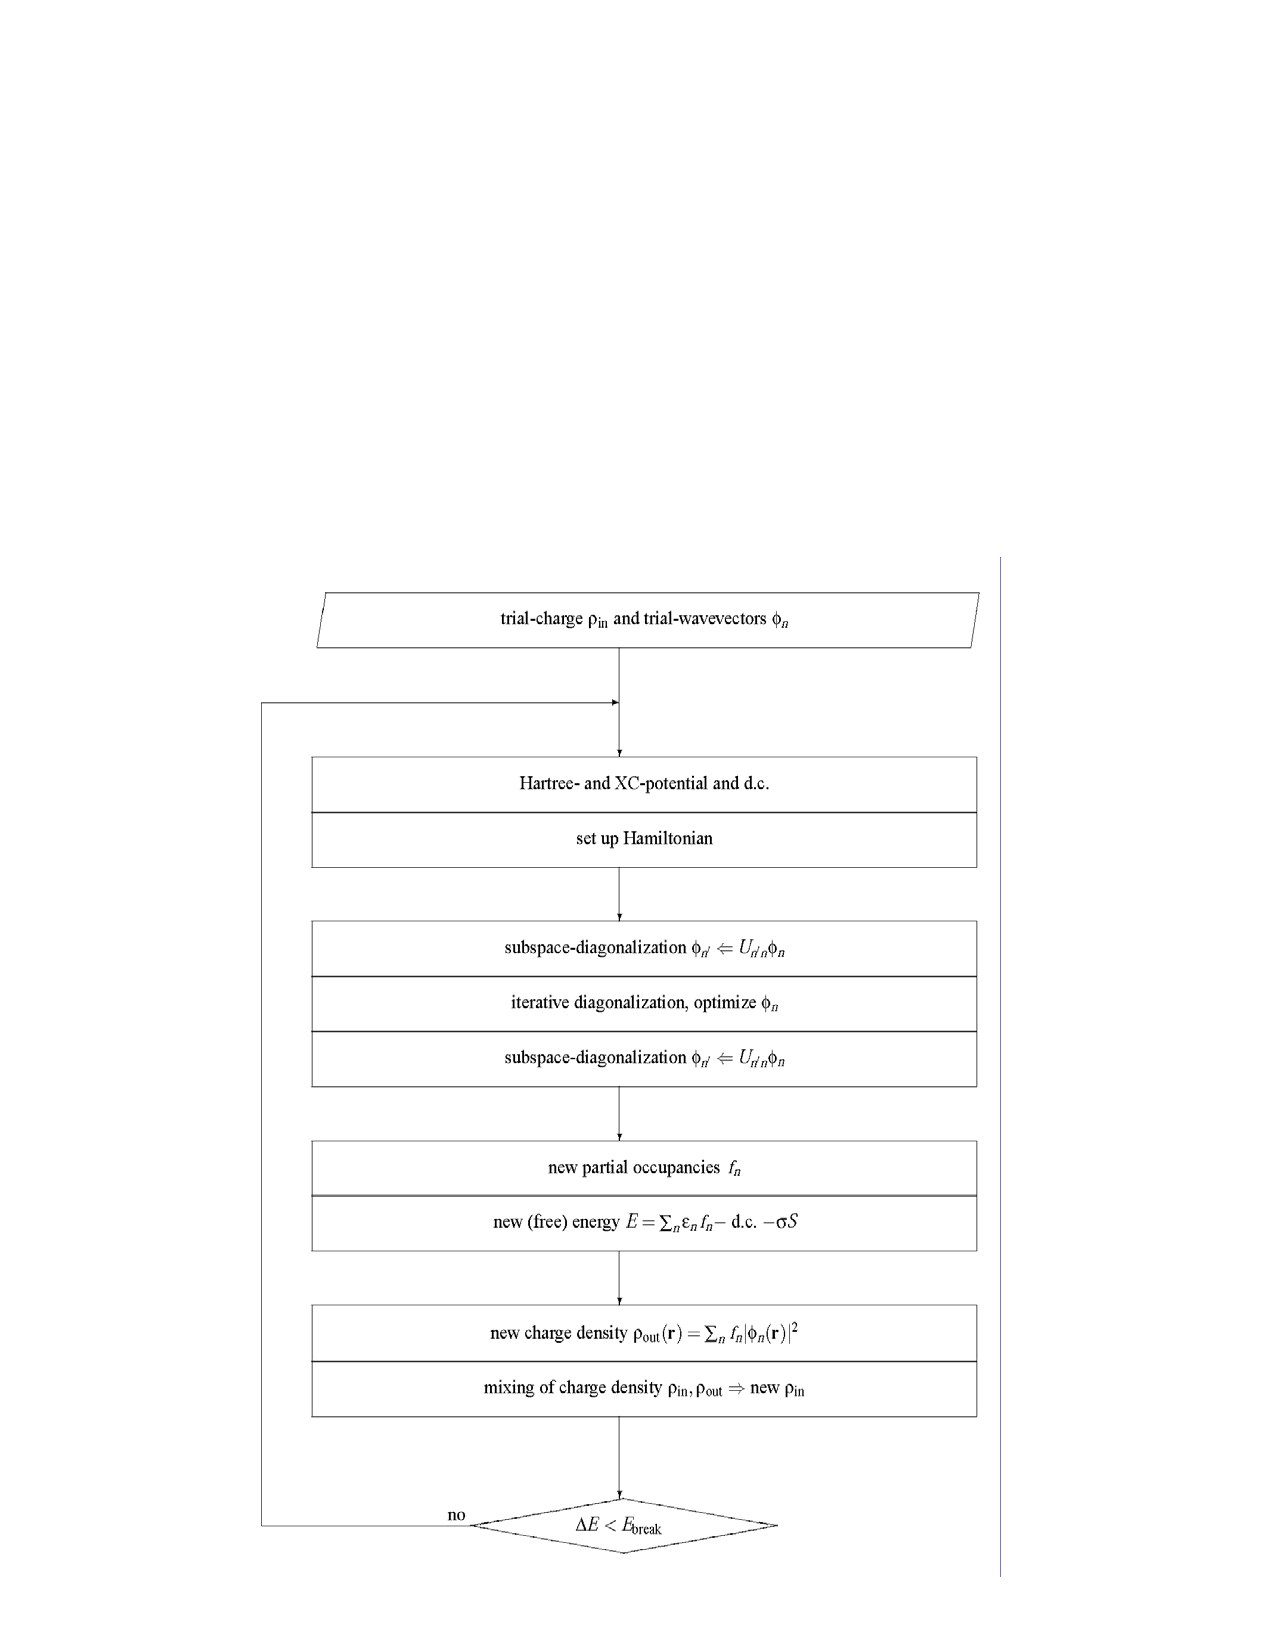
\includegraphics[height=3.0in,width=2.5in,viewport=125 42 474 555,clip]{Figures/VASP_Follow.pdf}
\caption{\small \textrm{Calculation of the K-S ground-states.}}%
\label{VASP_Follow}
\end{figure}
}

\frame
{
\frametitle{}
\begin{figure}[h!]
\centering
\vspace*{-0.80in}
%\hspace*{-10pt}
\includegraphics[height=3.72in,width=2.5in,viewport=160 118 395 755,clip]{Figures/VASP_main_Flow-1.eps}
\caption{\small \textrm{Calculation of the K-S ground-states.}}%
\label{VASP_Follow}
\end{figure}
}

\frame
{
\frametitle{}
\begin{figure}[h!]
\centering
\vspace*{-0.85in}
%\hspace*{-10pt}
\includegraphics[height=3.72in,width=2.5in,viewport=176 16 416 819,clip]{Figures/VASP_main_Flow-2.eps}
\caption{\small \textrm{Calculation of the K-S ground-states.}}%
\label{VASP_Follow}
\end{figure}
}

\frame
{
\frametitle{}
\begin{figure}[h!]
\centering
\vspace*{-0.85in}
%\hspace*{-10pt}
\includegraphics[height=3.72in,width=2.5in,viewport=146 173 416 812,clip]{Figures/VASP_main_Flow-3.eps}
\caption{\small \textrm{Calculation of the K-S ground-states.}}%
\label{VASP_Follow}
\end{figure}
}

\frame
{
\frametitle{}
\begin{figure}[h!]
\centering
\vspace*{-0.85in}
%\hspace*{-10pt}
\includegraphics[height=3.72in,width=2.5in,viewport=177 305 417 813,clip]{Figures/VASP_main_Flow-4.eps}
\caption{\small \textrm{Calculation of the K-S ground-states.}}%
\label{VASP_Follow}
\end{figure}
}

\section{$\vec k$空间积分与布点}
\frame
{
\frametitle{能带、\textrm{Fermi}面与$\vec k$空间积分}
\begin{figure}[h!]
\centering
\hspace{-0.5in}
\vspace{5.0in}
\subfigure[\footnotesize{Band structure}]{
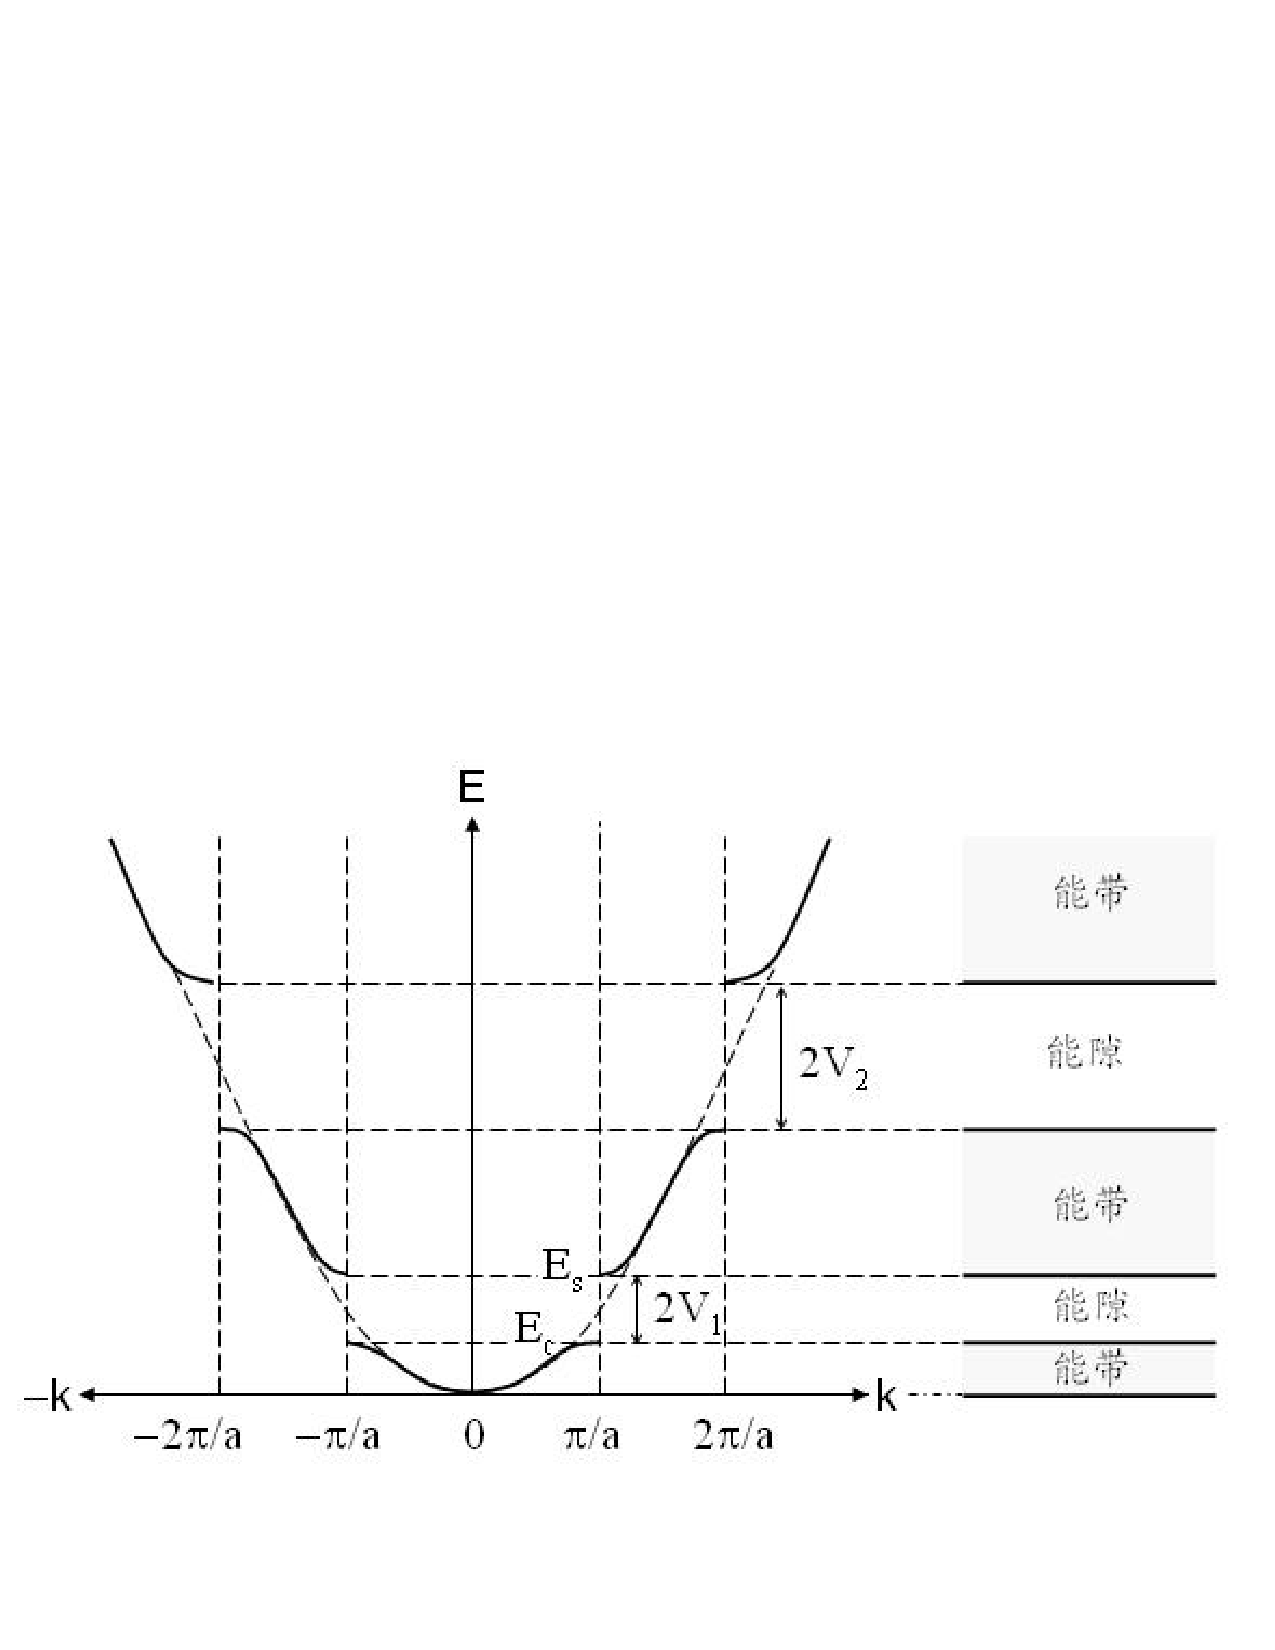
\includegraphics[height=1.4in,width=2.5in,viewport=10 90 570 380,clip]{Band_Gap.pdf}
%\caption{\small \textrm{}}%(与文献\cite{EPJB33-47_2003}图1对比)
%\label{Brillouin_Cube}
}
\subfigure[\footnotesize{Brillouin Zone}]{
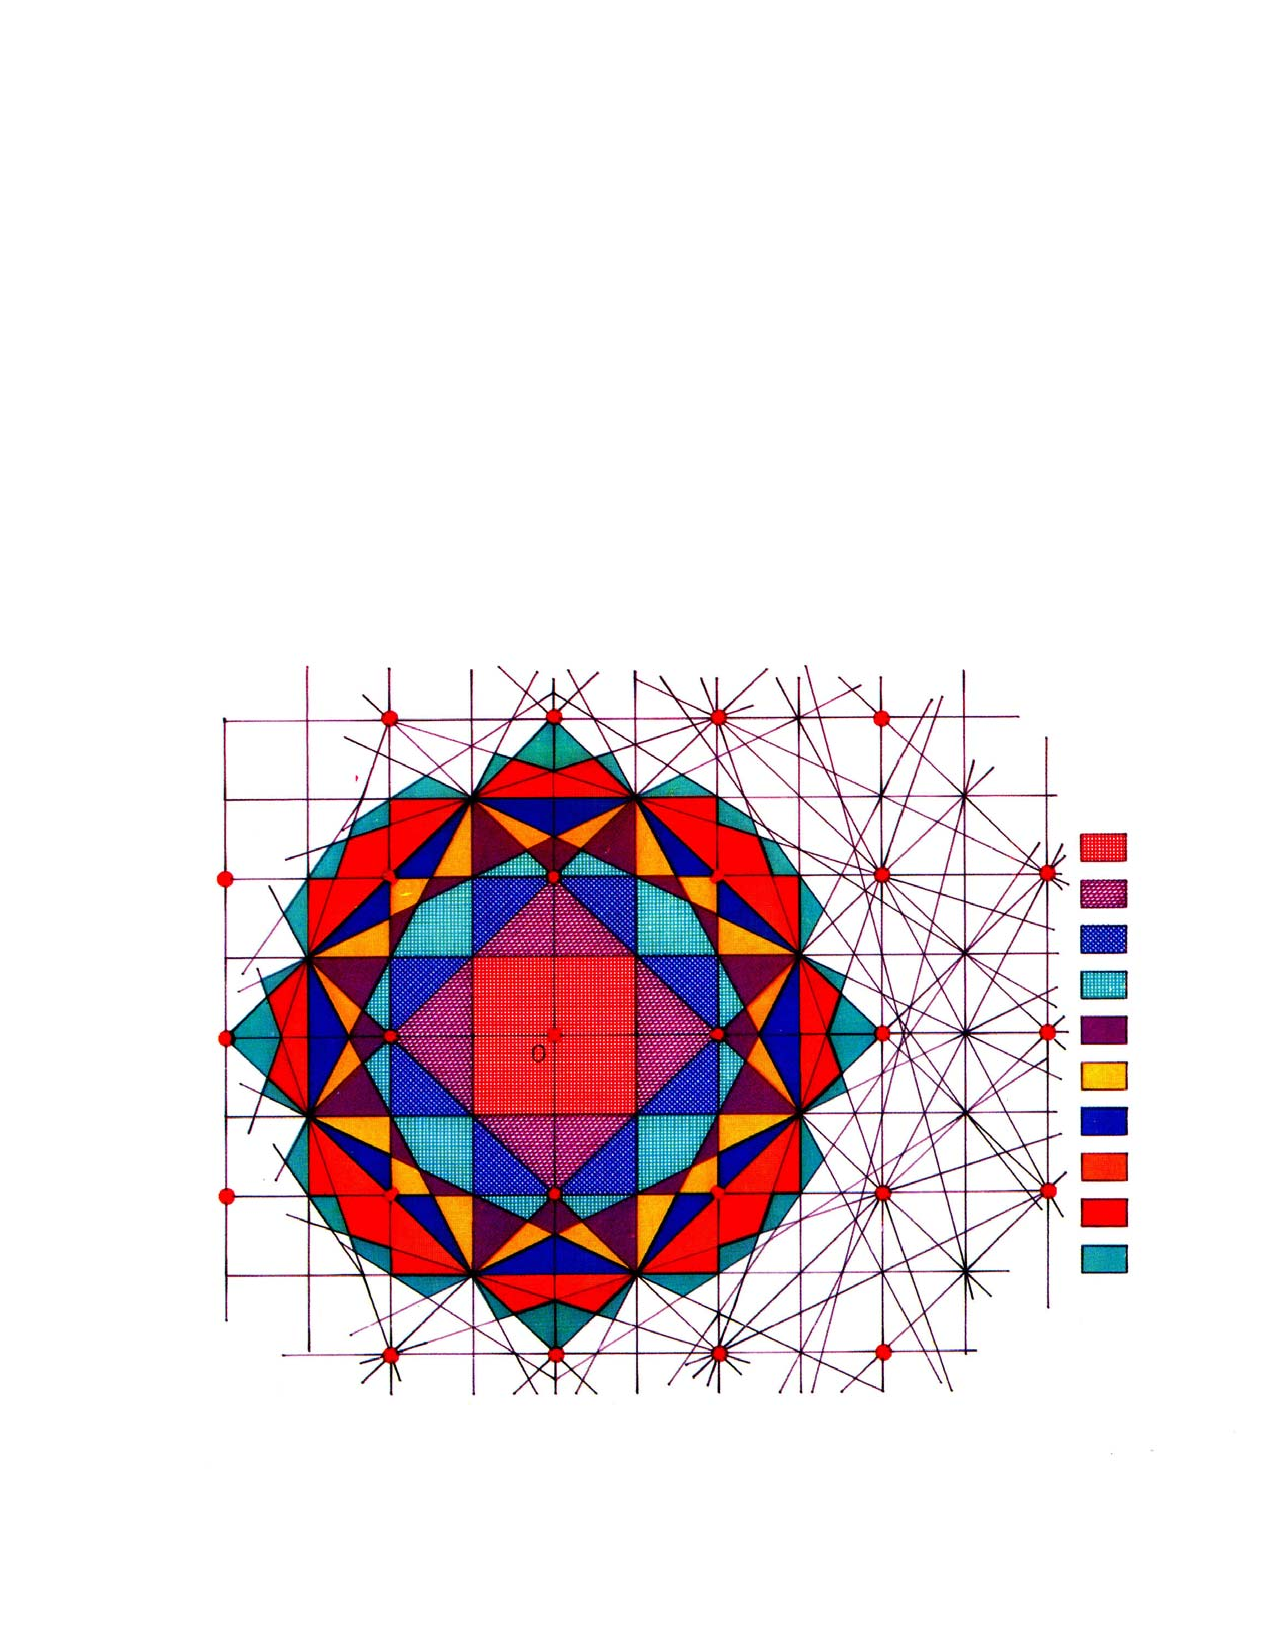
\includegraphics[height=1.28in,width=1.75in,viewport=100 120 545 470,clip]{2D_Brillouin-Zone.pdf}
%\caption{\small \textrm{}}%(与文献\cite{EPJB33-47_2003}图1对比)
%\label{Brillouin_Cube}
}
\end{figure}
}

\frame
{
\frametitle{$\vec k$ 空间布点方案}
\vskip 10pt
周期性体系计算,涉及除了在每个格点上求解\textrm{Schr\"odinger}方程外,计算固体性质的时还需要对$\vec k$空间中完成数值积分。
%\textbf{期望值},$\vec k$空间布点数值测试
\vskip 10pt
\begin{itemize}%[+-| alert@+>]
%\begin{enumerate}%[+-| alert@+>]
%\item $\vec k$空间布点方案
%  \begin{enumerate}
%\setlength{\itemsep}{15pt}
    \item 特殊点布点方案\textrm{(spectial points method)}\\
      将\textrm{Brillouin}区的积分变成网格点的权重求和
    \item 四面体布点方案\textrm{(tetrahedron method)}\upcite{PRB49-16233_1994}\\
	    \textrm{Brillouin}区积分转换为对网格点构成的四面体求和
%  \end{enumerate}
\end{itemize}
\begin{figure}[h!]
\centering
\vspace*{-0.2in}
\subfigure[\footnotesize{Special points}]{
\includegraphics[height=1.28in,width=1.24in,viewport=65 175 525 650,clip]{Special-points-1.eps}
%\caption{\small \textrm{}}%(与文献\cite{EPJB33-47_2003}图1对比)
%\label{Brillouin_Cube}
}
\subfigure[\footnotesize{Tetrahedron}]{
\includegraphics[height=1.28in,width=1.75in,viewport=40 125 525 465,clip]{Tetra-equal-ene.eps}
%\caption{\small \textrm{}}%(与文献\cite{EPJB33-47_2003}图1对比)
%\label{Brillouin_Cube}
}
\end{figure}
}

\frame
{
\frametitle{四面体布点积分方案}
\begin{itemize}
\setlength{\itemsep}{5pt}
	\item 对\textrm{WS}元胞用$N=(N_1+1)\times(N_2+1)\times(N_3+1)$个网格点(依次编号)分割为$N_1\times N_2\times N_3$个平行六面体
	\item 将每个平行六面体分为4个四面体,记下四面体顶点编号
\end{itemize}
\begin{figure}[h!]
\centering
\hspace*{-10pt}
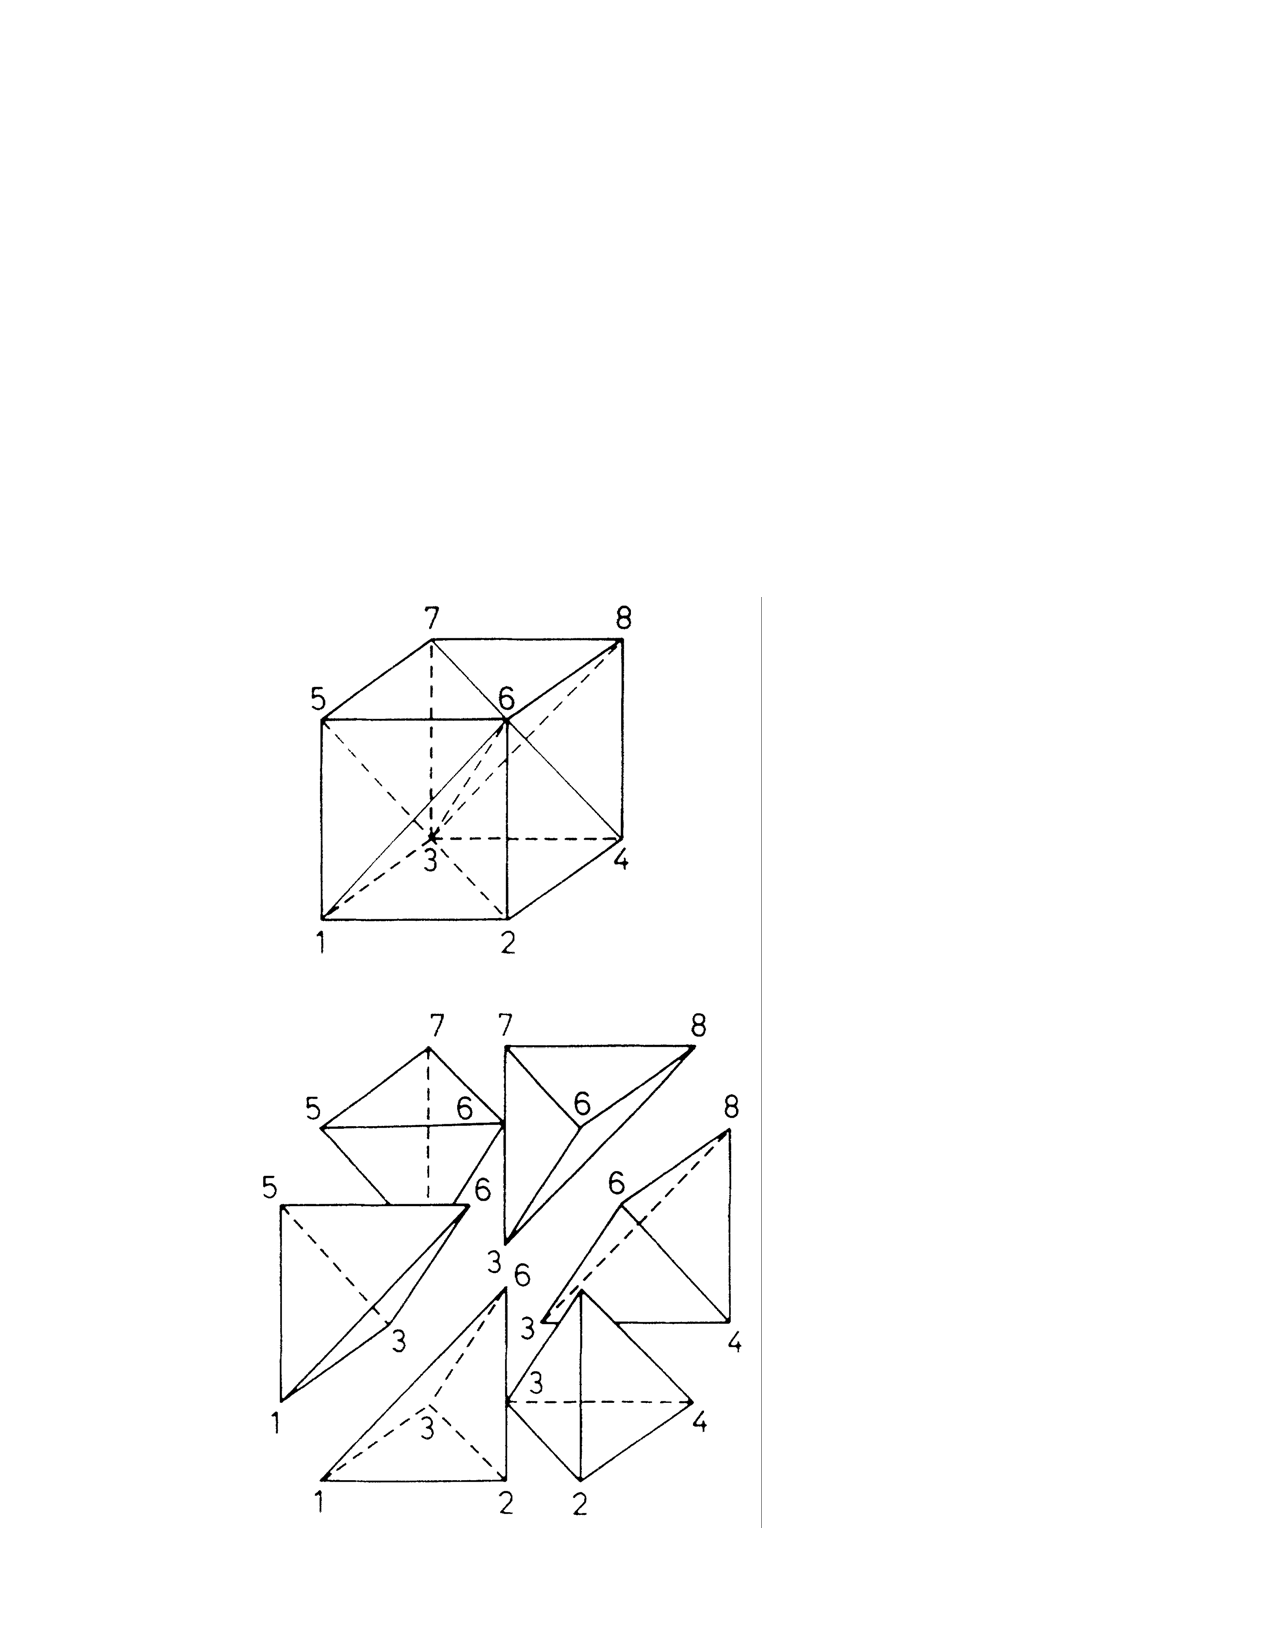
\includegraphics[height=1.8in,width=1.05in,viewport=120 60 360 505,clip]{submesh_Tetra.pdf}
\caption{\small \textrm{Breakup of a submesh cell into six tetrahedra.}}%(与文献\cite{EPJB33-47_2003}图1对比)
\label{Tetrahedron_split}
\end{figure}

}
\frame
{
\frametitle{四面体布点积分方案}
\begin{itemize}
\setlength{\itemsep}{10pt}
	\item 用点群对称性操作遍历全部网格点,各点对应的不可约第一\textrm{Brillouin}区\textrm{(Irreducible Brillouin zone, IBZ)}等价点标记
	\item 记录不可约\textrm{IBZ}的$\vec k$点及其权重
	\item 四面体中顶点编号全同的归为一类,同时统计各类四面体顶点序号和数目
\end{itemize}
每个四面体对$\vec k$-空间积分的权重表达式可参阅文献\cite{PRB49-16233_1994}
\begin{figure}[h!]
\centering
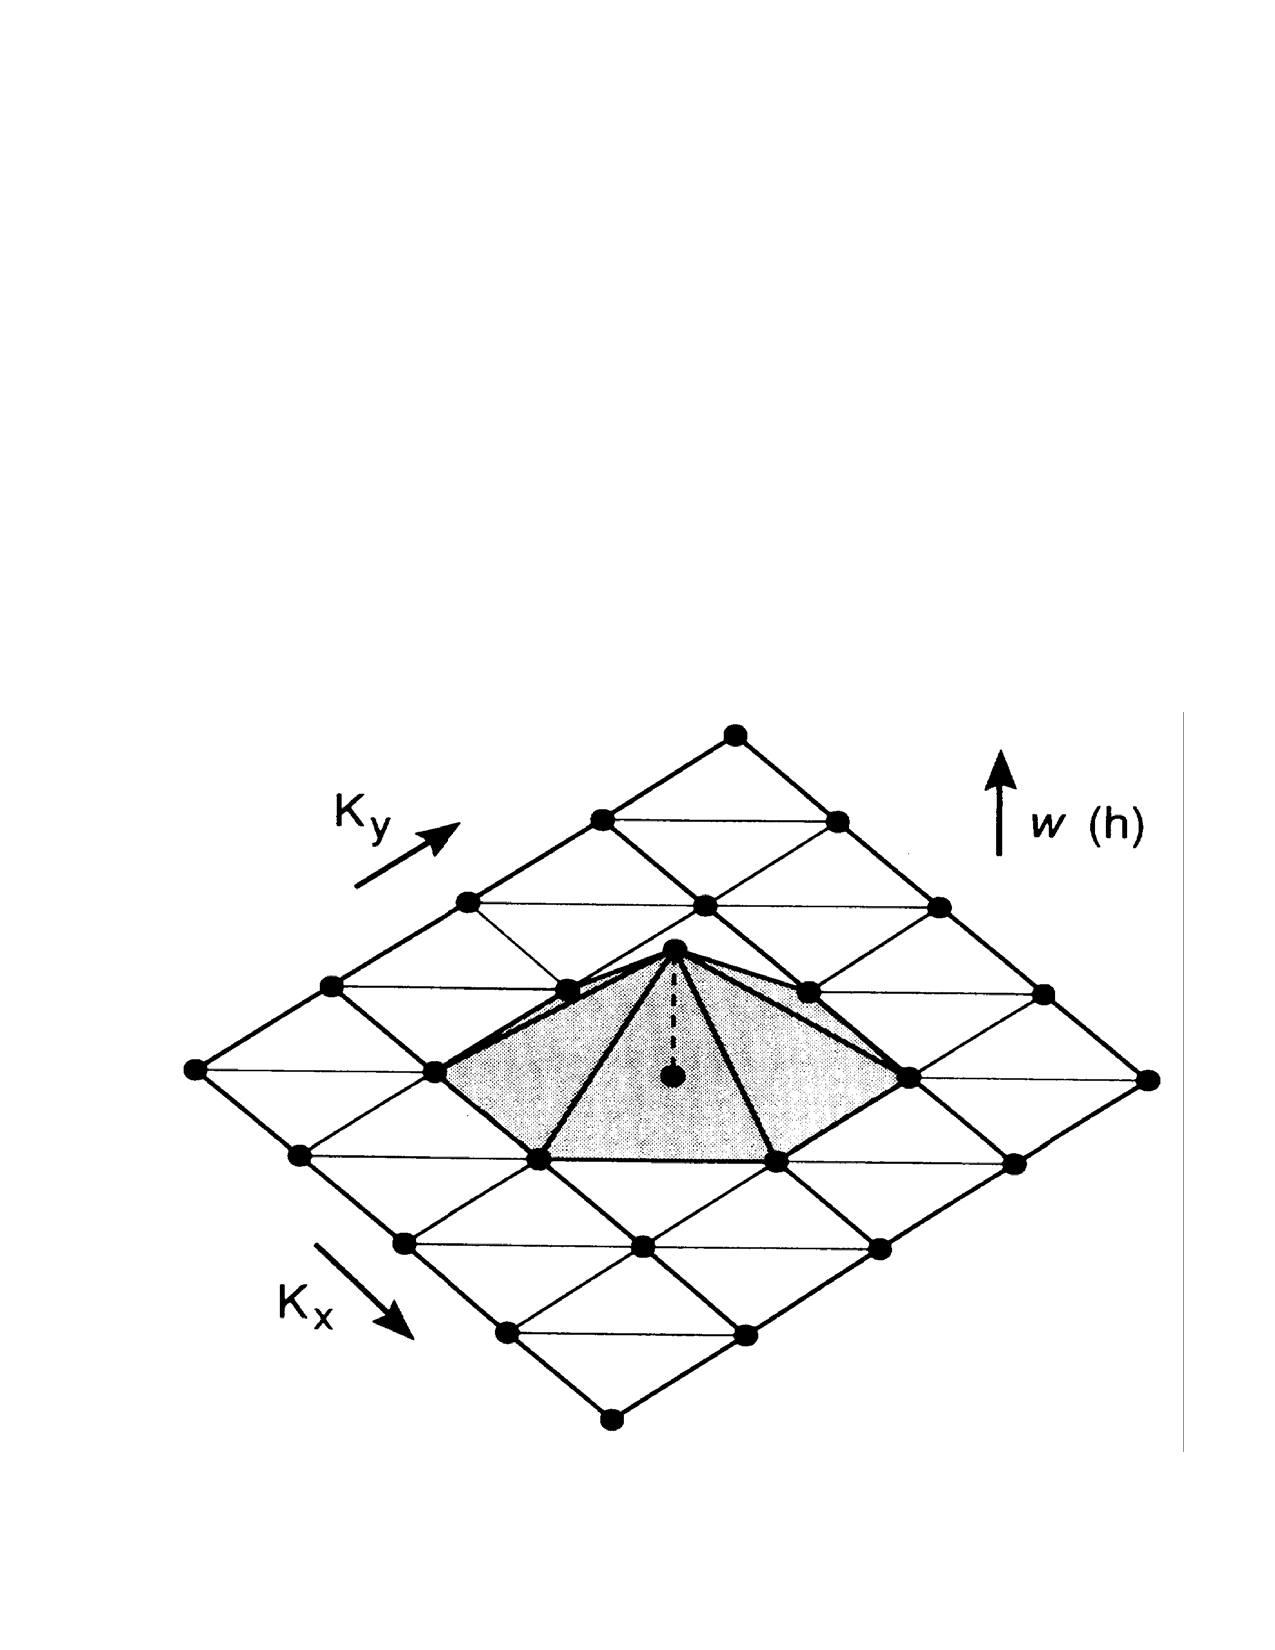
\includegraphics[height=0.95in,width=1.32in,viewport=85 99 560 460,clip]{dimen_Tetra.pdf}
\caption{\small \textrm{Two-dimensional schematic illustration of the functions $w_j(\vec k)$ that result in the integration weights when integrated.}}%(与文献\cite{EPJB33-47_2003}图1对比)
\label{Tetrahedron_weight}
\end{figure}
}

%\section{LDA+U与自相互作用的校正}
%\frame
%{
%\frametitle{LDA+U校正的基本思想}
%\begin{itemize}
%\setlength{\itemsep}{10pt}
%	\item 精确密度泛函具有当电子数在整数值前后改变的时候,体系能量的改变是不连续的属性,单电子能量的不连续对能带的带隙有很大贡献
%	 \item\textrm{LDA~}近似中体系能量是电子数的连续函数,不具备体系能量随电子数变化不连续的特征。\textrm{LDA/GGA~}方法在描述含有\textit{d}/\textit{f}电子的过渡金属和稀土元素化合物体系时常常失效。
%	\item \textrm{LDA}/\textrm{GGA~}得到的体系总能量和实验结果符合较好,但轨道能量(即$\varepsilon_i=\partial E/\partial n_i$),不符合\textrm{Koopmans~}定理,与实验或者严格计算得到的轨道能量差别很大%一个典型的例子就是对H原子的计算结果,LDA计算的轨道能级为$-$0.27\,a.u.(实验结果为$-$0.5\,a.u.),总能量($-$0.488\,a.u.)则非常接近$-$0.5\,a.u.\upcite{PRB37-9919_1988}。
%	\item \textrm{Anisimov~}提出通过对\textrm{LDA~}势加入轨道校正克服不足(称为\textrm{LDA+$U$}方法)\upcite{PRB44-943_1991,PRB48-16929_1993}%LDA+U方法与Andersen掺杂模型\upcite{PR124-41_1961}思想类似,
%\end{itemize}
%}
%\frame
%{
%\frametitle{$U$值的物理含义}
%\textrm{$U$}值的物理意义:含有$n$个3\textit{d}\,电子的原子中,\textrm{$U$}值定义为两个原子间转移一个\textit{d}\,电子的能量,即$$2(d^n)\rightarrow d^{n+1}+d^{n-1}$$
%\begin{figure}[h!]
%\centering
%\includegraphics[height=1.35in,width=2.32in,viewport=110 210 545 455,clip]{LDA_U.eps}
%\caption{\small \textrm{The meaning of $U$, when the Coulomb-interaction of each electron is taken into account.}}%(与文献\cite{EPJB33-47_2003}图1对比)
%\label{Tetrahedron_weight}
%\end{figure}
%}

%\frame
%{
%\frametitle{LDA+U近似处理含\textit{d}、\textit{f}电子的重元素体系}
%对局域的\textit{d}\,或\textit{f}\,电子,用含\textrm{$U$}的模型\textrm{Hamiltonian}考虑\textit{d}-\textit{d}或\textit{f}-\textit{f}间相互作用(定域\textrm{Coulomb}相互作用\textrm{$U$})。%,离域的\textit{s}\,和\textit{p}\,电子的运动用\textrm{LDA}近似描述。
%\begin{itemize}
%\setlength{\itemsep}{10pt}
%	\item \textrm{LDA+$U$}方法最重要的特征:通过参数\textrm{$U$}校正\textrm{LDA}中的电子自相互作用,使单电子能量变化出现不连续。%计算表明LDA+U方法对含有定域强Coulomb相互作用的体系是有效的\upcite{PRB48-16929_1993,JPCS56-1521_1995,EPL36-551_1996}。无论
%	\item \textrm{LDA+$U$}方法是平均场近似,对含有近似芯层的局域4\textit{f}\,电子的镧系元素离子还是过渡金属的氧化物(金属的3\textit{d}\,电子与氧原子2\textit{p}\,电子有很强的相互作用)体系都有效。如\textrm{FeSi}和\textrm{LaCaO$_3$}等体系,\textrm{LDA+$U$}能给出有关于金属-绝缘体转变的有用信息。甚至用于含有5\textit{f}\,电子的化合物的研究也取得一定的成功。
%\end{itemize}
%}

%\section{物理性质的计算}
%\frame
%{
%\frametitle{光学性质计算}
%\begin{itemize}
%\setlength{\itemsep}{10pt}
%	\item 半经典方法处理周期性体系的光学性质,用量子力学处理介质,对电磁波仍然采用经典电动力学描写。\upcite{Huang_Han}
%	\item 以半导体中的带间垂直跃迁(价带$|v,\vec k\rangle$,导带$|c,\vec k\rangle$)为例讨论固体的能带间跃迁。,晶体中动量为$\vec p$的电子在电磁场(电磁场矢量势为$\vec A$)存在情况下,应用含时微扰理论,准确到$\vec A$的线性项(忽略$\vec A$的平方项)
%微扰\textrm{Hamiltonian}为:
%\begin{displaymath}
%  H^{\prime}=\dfrac{\vec A}c\cdot\vec p
%  \label{eq:optic-25}
%\end{displaymath}
%	\item 频率为$\omega$的平面偏振光,电场和磁场的强度为
%\begin{displaymath}
%  \left\{
%\begin{aligned}
%    \vec E&=-\frac1c\frac{\partial\vec A}{\partial t}\\
%    \vec B&=\nabla\times\vec A
%  \end{aligned}%\right.
%  \label{eq:optic-26}
%\end{displaymath}
%\end{itemize}
%式中$c$为光速。
%}
%\frame
%{
%\frametitle{光学性质的计算}
%在含时微扰\textrm{Hamiltonian}作用下,只考虑吸收,跃迁几率为
%\begin{displaymath}
%  W=2\pi|\langle c,\vec k\,'|H'|v,\vec k\rangle|^2\delta[E_c(\vec k\,')-E_v(\vec k)-\omega]
%  \label{eq:optic-27}
%\end{displaymath}
%$\delta$因子表示跃迁过程的能量守恒关系%,矩阵元$\langle c\vec k|H'|v\vec k\rangle$表示\textrm{Bloch}函数间的积分
%。对垂直跃迁,忽略磁场贡献,%矩阵元可以简写成$\dfrac1cA_0\vec e\cdot\vec M_{cv}(\vec k)$,$\vec s$为电磁波矢量势$\vec A_0(=A_0\vec s)$方向的单位矢量。
%只有满足能量守恒和动量守恒条件的跃迁才对积分有贡献。%$\displaystyle\int W\dfrac{\textrm{d}\vec k}{(2\pi)^3}$为单位体积、单位时间内吸收能量为$\omega$的光子的总数,系数2是考虑两种自旋态。将式\eqref{eq:optic-27},\eqref{eq:optic-28}代入式\eqref{eq:optic-29},并应用$\dfrac{A_0}c\vec e\cdot\vec M_{cv}(\vec k)$表示矩阵元,得
%介质的能量吸收表达式
%\begin{displaymath}
%  \varepsilon_2(\omega)=2\left(\frac{2\pi}{\omega}\right)^2\sum_{v,c}\int|\vec e\cdot\vec M_{cv}(\vec k)|^2\delta[E_c(\vec k)-E_v(\vec k)-\omega]\frac{\textrm{d}\vec k}{(2\pi)^3}
%  \label{eq:optic-32}
%\end{displaymath}
%即描述能带间跃迁的$\varepsilon(\omega)$微观表达式,是晶体的光学吸收和能带结构之间的基本关系。
%对应的$\varepsilon_1$可以根据\textrm{Kramers-Kr\"onig}关系%\eqref{eq:optic-16}
%得到
%\footnotesize{\begin{displaymath}
%  \varepsilon_1(\omega)=1+8\pi\sum_{v,c}\int\frac{|\vec e\cdot\vec M_{cv}(\vec k)|^2}{[E_c(\vec k)-E_v(\vec k)][E_c(\vec k)-E_v(\vec k)]^2-\omega^2}\textrm{d}\vec k\frac2{(2\pi)^3}
%  \label{eq:optic-35}
%\end{displaymath}}
%}
%\frame
%{
%\frametitle{联合态密度(Joint DOS, JDOS)}
%定义联合态密度(\textrm{Joint Density of States, JDOS})
%\begin{displaymath}
%  J_{cv}(\hbar\omega)=\sum_{v,c}\int\delta[E_c(\vec k)-E_v(\vec k)-\omega]\frac{2\textrm{d}\vec k}{(2\pi)^3}
%  \label{eq:optic-33}
%\end{displaymath}
%\footnotesize{令$E_{cv}(\vec k)$\,=\,$E_c(\vec k)-E_v(\vec k)$,因$\textrm{d}\vec k$\,=\,$\dfrac{dE_{cv}(\vec k)}{\nabla_{\vec k}E_{cv}(\vec k)}\textrm{d}S$,故有
%\begin{displaymath}
%  J_{cv}(\omega)=\frac2{(2\pi)^3}\sum_{v,c}\int\limits_{E_{cv}(\vec k)=\omega}\frac{\textrm{d}S}{\nabla_{\vec k}E_{cv}(\vec k)}
%  \label{eq:optic-34}
%\end{displaymath}
%类似态密度的定义,而$E_{cv}(\vec k)$同时联系着价带和导带,因此称为联合态密度。当矩阵元$\vec M_{cv}(\vec k)$随波矢$\vec k$变化比较小的时候,可以近似地认为$\varepsilon_2(\omega)\!\propto\!J_{cv}(\omega)$。满足$|\nabla_{\vec k}E_{cv}(\vec k)|\!=\!0$的$\vec k$点,是联合态密度$J_{cv}(\omega)$和$\varepsilon_2(\omega)$的奇点(\textrm{Van Hove}奇点或临界点),在这些点,$J_{cv}(\omega)$和$\varepsilon_2(\omega)$%的能谱图将出现典型结构(即
%对能量的微商呈现典型的不连续。%联合态密度的奇点有两种情况,即$\nabla_{\vec k}E_c(\vec k)\!=\!\nabla_{\vec k}E_v(\vec k)\!=\!0$和$\nabla_{\vec k}E_c(\vec k)\!=\!\nabla_{\vec k}E_v(\vec k)\!\neq\!0$。将$E_{cv}(\vec k)$在奇点作Taylor级数展开到二级,$$E_{cv}(\vec k)=E_0+a_xk_x^2+a_yk_y^2+a_zk_z^2$$可以看出有四种类型的奇点:
%}}
%\frame
%{
%\frametitle{光学函数间的基本关系}
%\begin{itemize}
%	\item 电磁波在介质中传播,考虑介质的影响,速度为$c/n$,其中$n=\sqrt\varepsilon$为折射率。%类似的,
%	\item 考虑介质吸收,折射率$n$用复数$N=n+ik$表示,有$(n(\omega)+ik(\omega))^2=\varepsilon_1(\omega)+i\varepsilon_2(\omega)$,即$N^2=\varepsilon$。由此可得关系式:
%\begin{displaymath}
%  \left\{
%\begin{aligned}
%   \varepsilon_1(\omega)&=n(\omega)^2-k(\omega)^2\\
%   \varepsilon_2(\omega)&=2n(\omega)k(\omega)
% \end{aligned}%\right.
%  \label{eq:optic-9}
%\end{displaymath}
%相应地,
%\begin{displaymath}
%  \left\{
%\begin{aligned}
%   n^2&=\frac{\sqrt{\varepsilon_1^2+\varepsilon_2^2}+\varepsilon_1}2\\
%   k^2&=\frac{\sqrt{\varepsilon_1^2+\varepsilon_2^2}-\varepsilon_1}2
%   \end{aligned}%\right.
%  \label{eq:optic-10}
%\end{displaymath}
%	\item 因此用$\varepsilon_1$,$\varepsilon_2$或用$n$,$k$描述固体的光学性质是等价的。
%\end{itemize}
%}

\appendix






%------------------------------------------------------------------------Reference----------------------------------------------------------------------------------------------
%\begin{thebibliography}{99}
%-----------------------------------------------------------------------------------------------------------------------------------------------------------------------%
%\frame
%{
%\frametitle{主要参考文献}
%{\small
%\bibitem{Singh_Book}\textrm{D. J. Singh. \textit{Plane Wave, PseudoPotential and the LAPW method} (Kluwer Academic, Boston,USA, 1994)}					%
%  \nocite{*}																				%
%}
%}
%\end{thebibliography}
\begin{thebibliography}{99}
\frame
{
\frametitle{主要参考文献}
{\small
\bibitem{PR136-B864_1964}\textrm{P. Hohenberg and W. Kohn \textit{Phys. Rev.} \textbf{136} (1964), B864}
\bibitem{PR140-A1133_1965}\textrm{W. Kohn and L.J. Sham \textit{Phys. Rev.} \textbf{140} (1965), A1133}
\bibitem{Huang_Han}\textrm{黄昆 原著、韩汝琦 改编, \textit{固体物理学} 高等教育出版社, 北京, 1988}
\bibitem{Singh_Book}\textrm{D. J. Singh. \textit{Plane Wave, PseudoPotential and the LAPW method} (Kluwer Academic, Boston,USA, 1994)}
\bibitem{PRB41-7892_1990}\textrm{D. Vanderbilt. \textit{Phys. Rev.} B, \textbf{41} (1990), 7892} 
\bibitem{JPCM6-8245_1994}\textrm{G. Kresse and J. Hafner. J. Phys: \textit{Condens. Matter}, \textbf{6} (1994), 8245}
\bibitem{PRB50-17953_1994}\textrm{P. E. Bl\"ochl. \textit{Phys. Rev.} B, \textbf{50} (1994), 17953}
\bibitem{PRB59-1758_1999}\textrm{G. Kresse and D. Joubert \textit{Phys. Rev.} B, \textbf{59} (1999), 1758}
\bibitem{SSC114-15_2000}\textrm{E. Sj\"ostedt, L. Nordstr\"om and D. J. Singh. \textit{Solid State Commun.}, \textbf{114} (2000), 15}
\bibitem{WIEN2k_UG}\textrm{P. Blaha, K. Schwarz, G. Madsen, D. Kvasnicka and J. Luitz. \textit{User's Guide of WIEN2K, An Augmented Plane Wave Plus Local Orbitals Program for Calculating Crystal Properties}. Vienna University of Technology, Inst. of Physical and Theoretical Chemistry, Vienna, Austria (2012)}
\nocite*{}
}
%{\small
%\phantomsection\addcontentsline{toc}{section}{Bibliography}	 %直接调用\addcontentsline命令可能导致超链指向不准确,一般需要在之前调用一次\phantomsection命令加以修正	%
%\bibliography{Myref}																			%
%\bibliographystyle{mybib}																		%
%  \nocite{*}																				%
%}
%-----------------------------------------------------------------------------------------------------------------------------------------------------------------------%
}

\frame
{
\frametitle{主要参考文献}
{\small
%\bibitem{VASP_UG}\textrm{G. Kresse, M. Marsman, and J\"urgen Furthm\"uller. \textit{VASP the GUIDE}. Computational Physics, Faculty of Physics, Universit\"at Wien, Austria (2012) \\url http://cms.mpi.univie.ac.at/VASP/}
\bibitem{Comp_Method}\textrm{V. V. Nemoshkalenko and V. N. Antonov. \textit{Computational Methods in Solid State Physics} (Gordon and Breach Science Publisher, Amsterdam, The Netherlands, 1998)}
\bibitem{JMP22-2433_1981}\textrm{M. Weiner. \textit{J. Math. Phys.}, \textbf{22} (1981), 2433}
\bibitem{PRB26-4571_1982}\textrm{M. Weinert, E. Wimmer and A. J. Freeman. \textit{Phys. Rev.} B, \textbf{26} (1982), 4571}
\bibitem{PRB49-16233_1994}\textrm{P. E. Bl\"ochl, O. Jepsen and O. K. Andersen. \textit{Phys. Rev.} B, \textbf{49} (1994), 16233}
\bibitem{PRB44-943_1991}\textrm{V. I. Anisimov, J. Zaanen and O.K. Andersen. \textit{Phys. Rev.} B, \textbf{44} (1991), 943}
\bibitem{PRB48-16929_1993}\textrm{V.I. Anisimov, I.V. Solovyev, M.A. Korotin, M.T. Czyzyk and G.A. Sawatzky. \textit{Phys. Rev.} B, \textbf{48} (1993), 16929}
\nocite{*}																				%
}
}
\end{thebibliography}

%-----------------------------------------------------------Beamer下不建议使用bib,因为涉及分页--------------------------------------------------------------------------%
%{\small
%\phantomsection\addcontentsline{toc}{section}{Bibliography}	 %直接调用\addcontentsline命令可能导致超链指向不准确,一般需要在之前调用一次\phantomsection命令加以修正	%
%\bibliography{Myref}																			%
%\bibliographystyle{mybib}																		%
%  \nocite{*}																				%
%}
%------------------------------------------------------------------------------------------------------------------------------------------------------------------------------%

%-------------------------------------------------------------------------Thanks------------------------------------------------------------------------------------------------
%\section{致谢}
%\frame
%{
%\frametitle{致$\quad$谢}
%\begin{itemize}
%    \setlength{\itemsep}{20pt}
%  \item 感谢本团队高兴誉、吴泉生、宋红州等各位老师参与的讨论
%  \item 感谢莫所长、宋主任以及软件中心各位老师和同事
%  \item 感谢王崇愚先生的帮助
%\end{itemize}
%}
\frame
{
\vskip 60 pt
%\hskip 10pt \textcolor{blue}{\Huge 感谢答辩委员会各位老师\,\textrm{!}}\\
\vskip 35 pt
\hskip 60pt \textcolor{blue}{\Huge \textrm{谢谢大家\:!}}
%\vskip 15 pt
%\hskip 40pt \textcolor{blue}{\Huge \textrm{for your attention\:!}}
}
%-------------------------------------------------------------------------------------------------------------------------------------------------------------------------------

\frame
{
\vskip 60 pt
\vskip 35 pt
\hskip 60pt \textcolor{blue}{\Huge \textrm{VASP}上机练习}
}

\clearpage
\end{document}
